% Informe: Implementación de Sumatorias — Cálculo Aplicado, UCU 2026-2
% Compilar con: tectonic informe/main.tex   (o importar la carpeta en Overleaf)
\documentclass[11pt,a4paper]{article}

\usepackage[utf8]{inputenc}
\usepackage[T1]{fontenc}
\usepackage[spanish,es-tabla]{babel}   % es-tabla: "Tabla" en vez de "Cuadro"
\usepackage{amsmath,amssymb}
\usepackage{graphicx}
\usepackage{booktabs}
\usepackage{float}
\usepackage[margin=2.5cm]{geometry}
\usepackage[hidelinks]{hyperref}
\usepackage{caption}
\usepackage{microtype}

% Las fórmulas en línea no se parten al final del renglón: TeX solo puede cortar
% dentro de $...$ en una relación o en un operador binario, así que basta con
% prohibir esos dos puntos de corte.
\relpenalty=10000
\binoppenalty=10000

\graphicspath{{figuras/}}
\captionsetup{width=0.9\textwidth,font=small}
\decimalpoint

\begin{document}

% ---------- Portada ----------
\begin{titlepage}
  \centering
  \vspace*{2cm}
  {\Large Universidad Católica del Uruguay\par}
  {\large Facultad de Ingeniería y Tecnología\par}
  {\large Departamento de Ciencias Exactas y Naturales\par}
  \vspace{2.5cm}
  {\LARGE\bfseries Errores de redondeo en sumatorias:\ asociatividad, orden de suma y cancelación catastrófica\par}
  \vspace{2cm}
  {\large Martín De León \quad Manuel Chouhy \quad Joaquín Riál\par}
  \vspace{2cm}
  {\large Cálculo Aplicado\par}
  {\large Docentes: Maglis Mujica \quad Candido De Oliveira\par}
  \vspace{1.5cm}
  {\large \textbf{[FECHA PENDIENTE]}\par}
  \vfill
\end{titlepage}

\begin{abstract}
% Máximo 300 palabras. Objetivo, metodología, resultados más relevantes, conclusión principal.
% Autosuficiente: se tiene que entender sin leer el resto.

Las propiedades conmutativa y asociativa de la suma no se conservan en la aritmética de punto
flotante que ejecuta una computadora. Este trabajo mide ese apartamiento sobre tres sucesiones cuyo
valor exacto se conoce o se puede acotar: $a_N = \sum_{k=1}^{N} (1 + b^{k} - b^{k})$, que vale $N$;
$b_N = \sum_{k=1}^{N} 1/(k(k+1))$, de forma cerrada $N/(N+1)$; y
$c_N = \sum_{k=1}^{N} 1/(\sqrt{k^{2}+1} + k)$, que admite la representación equivalente
$\sqrt{k^{2}+1} - k$. Los cálculos se implementaron en Python con acumulación explícita, sin
funciones de reducción de biblioteca, y las figuras y tablas se generan con una corrida del código.

Con doble precisión, el término $1 + b^{k} - b^{k}$ deja de aportar pasado el mayor $k$ con
$|b|^{k} < 2^{53}$, y ese umbral predicho coincidió con el medido salvo en $b = \pm 2$, la única
base cuyas potencias pisan exactamente ese borde y la única donde la agrupación de los paréntesis
cambia el resultado. El entero de ancho fijo
devuelve el valor correcto pese a desbordar, porque la aritmética módulo $2^{64}$ conserva la
estructura de anillo. El orden de acumulación separó cuatro algoritmos en dos grupos con más de dos
órdenes de magnitud de diferencia, y ordenar de menor a mayor módulo alcanzó para igualar a la suma
compensada de Kahan. La cota estadística $\sqrt{N}\,u$ contuvo los errores medidos, mientras que la
cota de peor caso $Nu$ los sobreestimó por más de tres órdenes de magnitud. En $c_N$ la cancelación
entre cantidades próximas sí degradó el resultado, y la cota $2k^{2}u$ acertó el $k$ exacto en que
el término colapsa.

La pérdida de precisión aparece cuando el sumando cae por debajo de la resolución local del formato,
y la elección del orden de acumulación y de la representación algebraica pesa más que la del
formato.
\end{abstract}

\clearpage

\tableofcontents
\clearpage

\section{Introducción}
\label{sec:introduccion}
% Planteo del problema, justificación, objetivos (general y específicos), estructura del informe.
% Tiene que ser más larga que el resumen.

La suma de números reales es conmutativa y asociativa. Esas dos propiedades permiten escribir una
sumatoria como $\sum_{k=1}^{N} x_k$ sin aclarar en qué orden se recorren los términos ni cómo se
agrupan los paréntesis: cualquier camino conduce al mismo valor. La aritmética que ejecuta una
computadora no ofrece esa garantía. Cada resultado intermedio debe caber en una cantidad fija de
bits, así que casi todas las operaciones redondean. Ese redondeo depende de los valores que llegan
a cada paso. Dos programas que calculan la misma sumatoria con distinto orden o distinto
agrupamiento son entonces dos algoritmos diferentes, y pueden devolver números diferentes
(Goldberg, 1991).

Esa distancia entre la propiedad algebraica y su implementación aparece en situaciones corrientes de
programación. Un mismo código puede dar resultados distintos al paralelizarse, al cambiar de
biblioteca o al reordenar un bucle. Una suma de muchos términos pequeños puede perder cifras
significativas sin que nada en el programa lo señale. El problema no se anuncia con un mensaje de
error: el cálculo termina, devuelve un número con quince dígitos y algunos de esos dígitos son
incorrectos. Detectarlo exige una referencia contra la cual medir el error y un modelo de los
mecanismos que lo producen. Ambos son objeto del análisis numérico del redondeo (Higham, 2002).

Este trabajo estudia ese fenómeno sobre tres sucesiones elegidas para hacerlo medible. La primera,
$a_N = \sum_{k=1}^{N} (1 + b^{k} - b^{k})$, vale exactamente $N$ en $\mathbb{R}$ para cualquier base
$b$, de modo que toda desviación observada proviene del cálculo y no del planteo. La segunda,
$b_N = \sum_{k=1}^{N} 1/(k(k+1))$, tiene forma cerrada $N/(N+1)$ y admite varias formas de
recorrerse y de escribirse, lo que permite comparar algoritmos contra un valor de referencia. La
tercera, $c_N = \sum_{k=1}^{N} 1/(\sqrt{k^{2}+1} + k)$, no tiene forma cerrada conocida pero sí una
representación algebraicamente equivalente, $\sqrt{k^{2}+1} - k$, expuesta a la cancelación entre
cifras próximas. Las tres comparten una condición: el resultado correcto se conoce de antemano o se
puede acotar, y sin esa condición el error no sería observable.

El objetivo general es determinar en qué condiciones las propiedades algebraicas de la suma dejan de
valer en la aritmética de una computadora, cuánto se aparta el resultado del valor exacto en cada
caso y qué explica ese apartamiento. De ahí se desprenden cinco objetivos específicos:

\begin{enumerate}
  \item Identificar a partir de qué tamaño de los sumandos la agrupación de los paréntesis altera el
  resultado de una suma, y contrastar el comportamiento del entero de precisión arbitraria de Python
  con el del punto flotante de doble precisión y con el del entero de ancho fijo.
  \item Medir cómo depende el error de una suma acumulada del orden en que se recorren los términos,
  comparando cuatro estrategias de acumulación sobre la misma serie, entre ellas la suma compensada
  de Kahan.
  \item Cuantificar la discrepancia entre representaciones algebraicamente equivalentes de una misma
  sumatoria y establecer cuándo la cancelación entre cantidades próximas degrada el resultado y
  cuándo resulta inofensiva.
  \item Contrastar cada medición con las cotas de error que predice el análisis teórico, y evaluar
  si describen el comportamiento observado o lo sobreestiman.
  \item Producir un conjunto de programas que genere todas las figuras y tablas del informe, de modo
  que cada dato presentado sea reproducible a partir del código.
\end{enumerate}

El informe se organiza en cinco secciones además de esta, más la bibliografía. La sección \ref{sec:marco} reúne los
conceptos necesarios para leer los resultados: la representación en punto flotante y sus dos
constantes de resolución, los enteros de precisión arbitraria, el estado de las propiedades
conmutativa y asociativa en la aritmética de máquina, la medida de error empleada, la suma de Kahan,
las sumas telescópicas y la cancelación catastrófica. Allí quedan enunciadas las cotas que después
se comparan contra los datos. La sección \ref{sec:metodologia} describe el entorno, el diseño de
cada experimento, los criterios de análisis, el tratamiento de la aleatoriedad y la ubicación del
código. La sección
\ref{sec:resultados} presenta las mediciones agrupadas por fenómeno y no por experimento: la pérdida
de la asociatividad, la dependencia del orden de suma y el comportamiento de representaciones
equivalentes. La sección \ref{sec:discusion} interpreta esas mediciones, las compara con las cotas
teóricas, examina dos resultados que contradicen la expectativa inicial y enuncia las limitaciones
del estudio. La sección \ref{sec:conclusiones} sintetiza las respuestas a los objetivos y señala
líneas de trabajo posteriores.

\section{Marco teórico}
\label{sec:marco}
% Una subsección por concepto clave, solo los que se usan. Cada afirmación fuerte con referencia.

\subsection{Representación en punto flotante}
\label{subsec:punto-flotante}

Una computadora almacena cada número real en una cantidad fija de bits, así que solo puede
representar un subconjunto finito de $\mathbb{R}$. El estándar IEEE~754 fija cómo se elige ese
subconjunto y cómo se redondean los resultados de las operaciones (Institute of Electrical and
Electronics Engineers [IEEE], 2019). Python usa el
formato de doble precisión, \texttt{binary64}, que reparte sus 64 bits en un bit de signo, 11 bits
de exponente y 52 bits de mantisa almacenada. Todo número normal del formato se escribe como
\begin{equation}
  x = (-1)^{s}\,(1.m_1m_2\ldots m_{52})_2 \times 2^{e},
  \qquad -1022 \le e \le 1023 ,
  \label{eq:binary64}
\end{equation}
donde el 1 inicial no se guarda. La mantisa tiene entonces 53 bits de precisión efectiva. El mayor
valor representable es del orden de $1.80 \times 10^{308}$ y el menor normal positivo, del orden de
$2.23 \times 10^{-308}$.

Llamamos $\mathbb{F}$ al conjunto de números representables y $\mathrm{fl}(x)$ al elemento de
$\mathbb{F}$ más próximo a $x$, con desempate al de mantisa par, que es el modo de redondeo por
defecto del estándar. Dos constantes describen la resolución del formato. La unidad de redondeo
$u = 2^{-53} \approx 1.11 \times 10^{-16}$ acota el error relativo de representar un real,
\begin{equation}
  \frac{|\mathrm{fl}(x) - x|}{|x|} \le u ,
  \label{eq:redondeo}
\end{equation}
y el épsilon de máquina $\varepsilon_{\mathrm{M}} = 2^{-52} \approx 2.22 \times 10^{-16}$ mide la
distancia entre 1 y el siguiente elemento de $\mathbb{F}$. La distinción importa porque las dos
constantes difieren en un factor 2 y la bibliografía usa las dos (Higham, 2002).

De \eqref{eq:redondeo} sale el modelo estándar del análisis de error de redondeo: si
$\mathrm{op}$ es una de las cuatro operaciones aritméticas o la raíz cuadrada, el estándar exige que
el resultado en máquina sea el redondeo del resultado exacto, de modo que
\begin{equation}
  \mathrm{fl}(x \mathbin{\mathrm{op}} y) = (x \mathbin{\mathrm{op}} y)(1 + \delta),
  \qquad |\delta| \le u .
  \label{eq:modelo}
\end{equation}
Cada operación introduce un error relativo acotado por $u$, y el análisis de un algoritmo consiste
en seguir cómo se acumulan esos $\delta$ (Higham, 2002).

El espaciado de $\mathbb{F}$ no es uniforme: dentro de la binada $[2^{e}, 2^{e+1})$ los elementos
están separados por $2^{e-52}$. Los enteros son un caso particular útil. Todos los enteros con
$|n| \le 2^{53}$ pertenecen a $\mathbb{F}$; por encima de $2^{53}$ el espaciado pasa a valer 2 y
solo se representan los pares. De ahí sale el techo que aparece en el experimento de la
asociatividad. Si $x \ge 2^{54}$, el 1 queda por debajo de medio espaciado y el redondeo lo
descarta, de modo que $\mathrm{fl}(1 + x) = x$. En la binada $[2^{53}, 2^{54})$, donde el
espaciado vale 2, el 1 vale exactamente medio espaciado y el resultado lo decide el desempate a
mantisa par: $\mathrm{fl}(1 + x) = x$ si $x$ es múltiplo de 4 y $\mathrm{fl}(1 + x) = x + 2$ si no
lo es. El caso que interesa acá es el primero, porque $x = 2^{53}$ es múltiplo de 4.

El límite tampoco es simétrico, y esa asimetría explica una de las anomalías del experimento. En
$[2^{52}, 2^{53})$ el espaciado es 1 y en $[2^{53}, 2^{54})$ es 2, así que $2^{53} - 1$ es
representable exacto y $2^{53} + 1$ no lo es. Restar primero deja el resultado en la binada de
abajo, que tiene el doble de resolución, y ahí el 1 sobrevive: $\mathrm{fl}(1 - 2^{53})$ vale
$-(2^{53} - 1)$ y no $-2^{53}$.

Cuando una operación produce un valor de módulo mayor que el máximo representable, el estándar
devuelve $\pm\infty$ en lugar de detener el cálculo. Las operaciones indeterminadas sobre esos
valores, como $\infty - \infty$, devuelven \texttt{NaN}, un dato especial que se propaga por el
resto de la cuenta y que no es igual a sí mismo (IEEE, 2019).

\subsection{Enteros de precisión arbitraria}
\label{subsec:enteros}

El tipo \texttt{int} de Python no tiene ancho fijo: cada entero usa tantas palabras de memoria como
necesite su magnitud, y las operaciones aritméticas entre enteros son exactas mientras haya memoria
disponible (Python Software Foundation, 2024). No hay desborde ni redondeo, así que las identidades
algebraicas que valen en $\mathbb{Z}$ valen también en el programa.

Lo que sí cambia es el costo. Un entero de valor $|n|$ ocupa del orden de $\log_2 |n|$ bits, de modo
que $b^{k}$ necesita unos $k \log_2 b$ bits. Multiplicar ese número por $b$ cuesta un tiempo
proporcional a su longitud, y calcular las potencias sucesivas hasta $k = N$ acumula un costo del
orden de $N^{2}$. La aritmética exacta se paga en tiempo y en memoria.

C y Java no ofrecen este tipo por defecto: el tipo entero habitual tiene 32 o 64 bits fijos, y un
resultado fuera de rango desborda. Las dos familias resuelven el desborde de manera distinta: el
estándar de C declara que el desborde de un entero con signo es comportamiento indefinido, es decir,
que el compilador no está obligado a producir ningún resultado en particular (International
Organization for Standardization [ISO], 2018), mientras que Java define el resultado como la
reducción módulo $2^{n}$ en complemento a dos, con $n$ el ancho del tipo. Los enteros de ancho fijo
de NumPy, como \texttt{int64}, siguen esta segunda convención, que para ese tipo es la reducción
módulo $2^{64}$.

Esa convención importa para leer los datos. La
aritmética módulo $2^{64}$ es la de un anillo, con lo cual sigue siendo asociativa, conmutativa y
distributiva de forma exacta. Un cálculo cuyas operaciones intermedias desbordan puede terminar en
el resultado correcto si la expresión final vuelve a caer dentro del rango representable, porque las
cifras que se perdieron por arriba se cancelan entre sí.

\subsection{Asociatividad y conmutatividad en aritmética de punto flotante}
\label{subsec:asociatividad}

En $\mathbb{R}$ la suma es conmutativa y asociativa, y por eso una sumatoria se escribe sin
paréntesis y sin indicar en qué orden se recorren los sumandos. La suma de punto flotante conserva
solo la primera de las dos propiedades. Es conmutativa porque $\mathrm{fl}(x + y)$ depende del valor
exacto de $x + y$ y de la función de redondeo, y las dos son simétricas en sus argumentos. No es
asociativa: con $x = 1$ e $y = 2^{53}$,
\begin{equation}
  \mathrm{fl}\bigl(\mathrm{fl}(1 + 2^{53}) - 2^{53}\bigr) = 0
  \quad\text{y}\quad
  \mathrm{fl}\bigl(1 + \mathrm{fl}(2^{53} - 2^{53})\bigr) = 1 .
  \label{eq:contraejemplo}
\end{equation}
Los dos miembros son el mismo cálculo con distinta agrupación de paréntesis y difieren en todo el
valor del término (Goldberg, 1991).

La distinción tiene una consecuencia directa sobre el experimento del orden de suma. Una suma
acumulada de $N$ términos es una secuencia encadenada de sumas binarias, y permutar los sumandos
equivale a evaluar un agrupamiento distinto de la misma expresión. Lo que se pone a prueba al
reordenar los términos es la asociatividad y no la conmutatividad: el resultado cambia porque la
suma de punto flotante no es asociativa.

Para la suma acumulada de $N$ términos del mismo signo, el análisis de peor caso da una cota de
error absoluto proporcional a $N u \sum_{k} |x_k|$, que se obtiene suponiendo que los $N-1$
redondeos se acumulan todos en la misma dirección (Higham, 2002). Es una cota conservadora. Si en
cambio se modelan los $\delta$ de \eqref{eq:modelo} como variables independientes de media nula, la
suma de los errores se comporta como un paseo aleatorio y el crecimiento típico del error relativo
resulta
\begin{equation}
  E_{\mathrm{rel}} \sim \sqrt{N}\,u ,
  \label{eq:cota-raiz}
\end{equation}
que es la referencia estadística con la que se comparan los datos de este trabajo (Higham, 2002).
Del mismo análisis se desprende que, para términos positivos, acumular de menor a mayor módulo
reduce el error: cada término chico se suma cuando el acumulador todavía es chico y su información
no cae por debajo del último bit de la mantisa.

\subsection{Error relativo}
\label{subsec:error-relativo}

Dado un valor teórico $x \ne 0$ y su aproximación numérica $\hat{x}$, el error relativo es
\begin{equation}
  E_{\mathrm{rel}} = \frac{|\hat{x} - x|}{|x|} .
  \label{eq:error-relativo}
\end{equation}
Es la medida natural en punto flotante porque la precisión del formato es relativa: según
\eqref{eq:redondeo}, el error de representación crece con la magnitud del número, pero su cociente
con esa magnitud queda acotado por $u$ en todo el rango. Como referencia de lectura, un error
relativo del orden de $10^{-d}$ corresponde a unas $d$ cifras decimales significativas correctas.

La interpretación de esta medida tiene dos límites. El valor teórico también
se evalúa en punto flotante, así que el piso de lo que se puede medir es del orden de $u$: un error
relativo nulo significa que el resultado coincide bit a bit con el valor de referencia calculado, no
que sea exacto. El error relativo también necesita una forma cerrada contra la cual
comparar. Cuando la sucesión no tiene una, lo que se compara son dos representaciones entre sí, y la
diferencia absoluta $D_N$ entre ellas mide la discrepancia de los dos cálculos, no el error de
ninguno de los dos.

\subsection{Suma de Kahan}
\label{subsec:kahan}

La suma compensada de Kahan reduce el error de la suma acumulada arrastrando de forma explícita la
parte del término que el redondeo descarta (Kahan, 1965). El algoritmo mantiene, además del
acumulador $s$, una variable de compensación $c$ que guarda el error de la iteración anterior. En
cada paso, con el término $x_k$, calcula
\begin{equation}
  y = x_k - c, \qquad
  t = s + y, \qquad
  c = (t - s) - y, \qquad
  s = t ,
  \label{eq:kahan}
\end{equation}
donde cada línea se evalúa en punto flotante. La clave está en la tercera: cuando $|s| \ge |y|$, la
expresión $(t - s) - y$ recupera exactamente el error de redondeo cometido al formar $t = s + y$, y
la iteración siguiente lo devuelve al cálculo restándoselo al término entrante.

La cota de error del algoritmo para $N$ términos es de la forma $2u + O(Nu^{2})$ veces
$\sum_k |x_k|$, es decir, prácticamente independiente de $N$ para los tamaños de este trabajo
(Higham, 2002). Frente a la cota $Nu$ de la suma acumulada, la ganancia crece con la cantidad de
términos. El costo es de cuatro operaciones de punto flotante por término en lugar de una. Queda
además una advertencia de implementación: un compilador o una biblioteca que reasocie las
expresiones de \eqref{eq:kahan} suponiendo que la suma es asociativa anula la compensación, porque
en $\mathbb{R}$ la variable $c$ vale idénticamente cero.

\subsection{Sumas telescópicas}
\label{subsec:telescopicas}

Una suma es telescópica cuando su término general se escribe como diferencia de dos valores
consecutivos de una misma sucesión, $x_k = t_k - t_{k+1}$. En ese caso los términos intermedios se
cancelan de a pares y queda
\begin{equation}
  \sum_{k=1}^{N} (t_k - t_{k+1}) = t_1 - t_{N+1} .
  \label{eq:telescopica}
\end{equation}
La sucesión $b_N = \sum_{k=1}^{N} 1/(k(k+1))$ es de este tipo, con $t_k = 1/k$, porque la
descomposición en fracciones simples da $1/(k(k+1)) = 1/k - 1/(k+1)$. Aplicando
\eqref{eq:telescopica} se obtiene la forma cerrada
\begin{equation}
  b_N = 1 - \frac{1}{N+1} = \frac{N}{N+1} .
  \label{eq:forma-cerrada}
\end{equation}

Las cuatro expresiones anteriores son la misma en $\mathbb{R}$ y describen cuatro programas
distintos en $\mathbb{F}$. La suma del producto evalúa una división y una suma por término; la
telescópica evalúa dos divisiones y una resta antes de acumular; y las dos formas cerradas de
\eqref{eq:forma-cerrada} difieren en la cantidad de redondeos, una división y una resta contra una
sola división. Por \eqref{eq:modelo}, cada operación agrega su propio $\delta$, así que las cotas de
error de las cuatro no tienen por qué coincidir, y tampoco sus resultados.

\subsection{Cancelación catastrófica}
\label{subsec:cancelacion}

La cancelación catastrófica es la pérdida de cifras significativas que ocurre al restar dos números
de punto flotante próximos entre sí (Goldberg, 1991). Si los operandos llegan a la resta con errores
relativos $\delta_1$ y $\delta_2$ heredados de cálculos anteriores, el error relativo del resultado
queda acotado por
\begin{equation}
  \frac{|\widehat{x - y} - (x - y)|}{|x - y|}
  \le \frac{|x| + |y|}{|x - y|} \max(|\delta_1|, |\delta_2|) ,
  \label{eq:amplificacion}
\end{equation}
y el factor $(|x| + |y|)/|x - y|$ crece sin cota cuando $x$ e $y$ se acercan. Las cifras altas, que
eran correctas, se cancelan entre sí; las cifras bajas, que ya estaban contaminadas, quedan al
frente del resultado.

El nombre del fenómeno sugiere que el error lo introduce la resta, y no es así. El lema de Sterbenz
establece que si $x$ e $y$ son positivos y cumplen
$y/2 \le x \le 2y$, entonces $x - y$ pertenece a $\mathbb{F}$ y la resta se calcula sin error
(Sterbenz, 1974). Es decir que en el régimen donde la cancelación es más severa la resta suele ser
exacta: no crea error nuevo, expone el que traían los operandos.

La sucesión $c_N = \sum_{k=1}^{N} 1/(\sqrt{k^{2}+1} + k)$ ilustra el mecanismo. Su término general
admite la representación equivalente $\sqrt{k^{2}+1} - k$, que se obtiene multiplicando y dividiendo
por el conjugado. Para $k$ grande, $\sqrt{k^{2}+1} \approx k\,(1 + 1/(2k^{2}))$, de modo que los dos
operandos de la resta están dentro de un factor 2 y el lema de Sterbenz se aplica. El único error lo
aporta el redondeo previo de la raíz, de tamaño relativo $u$ y por lo tanto de tamaño absoluto del
orden de $k u$. Como el valor exacto de la diferencia es cercano a $1/(2k)$, el error relativo del
término calculado por la resta resulta del orden de
\begin{equation}
  \frac{k u}{1/(2k)} = 2k^{2} u ,
  \label{eq:cota-termino}
\end{equation}
una cota que crece cuadráticamente con $k$ y que alcanza el valor 1, es decir la pérdida completa de
las cifras significativas, en $k = 1/\sqrt{2u} = 2^{26}$. De ahí se desprende una cota para la suma
completa. Cada término aporta un error absoluto del orden de $k u$, de modo que si los errores de
los $N$ términos se alinearan en la misma dirección la discrepancia acumulada sería del orden de
$\sum_{k \le N} k u \approx N^{2} u / 2$, y crecería cuadráticamente con $N$. En lo que sigue se
usa la forma redondeada $N^{2}u$, que es el doble de esa estimación y por lo tanto la acota. Es el
análogo de la cota $Nu$ de la suma acumulada: describe el peor caso y no el típico. La representación como cociente suma en el
denominador en lugar de restar, así que no hay cancelación y su error relativo se mantiene del orden
de $u$ para todo $k$. La recomendación general es la de Goldberg (1991): frente a dos expresiones
algebraicamente equivalentes conviene elegir la que evita la resta de cantidades próximas, y la
racionalización por el conjugado es la transformación habitual para conseguirlo.

\section{Metodología}
\label{sec:metodologia}
% Herramientas y versiones, diseño de cada experimento, criterios de análisis, semilla,
% uso de Claude, y el link al repositorio (SOLO acá).

\subsection{Entorno y herramientas}
\label{subsec:entorno}

Todo el trabajo numérico se hizo en Python 3.12.3 sobre Windows 11, con NumPy 1.26.4 (Harris
et al., 2020) para los arreglos y los generadores de números aleatorios, y Matplotlib 3.11.1
(Hunter, 2007) para las figuras. El tipo \texttt{float} de Python corresponde al formato
\texttt{binary64} descrito en la sección \ref{subsec:punto-flotante}, y el tipo \texttt{int} es el
entero de precisión arbitraria de la sección \ref{subsec:enteros}. Las dos únicas dependencias
externas están declaradas en \texttt{requirements.txt} con sus versiones mínimas. El informe se
escribió en \LaTeX{} y se compiló con Tectonic.

Ninguna sumatoria del trabajo usa la función \texttt{sum()} de Python ni las reducciones de NumPy.
Los términos se acumulan siempre con un ciclo \texttt{for} explícito.
El objeto de estudio es el orden en que se encadenan las sumas parciales, y una reducción de
biblioteca puede agrupar los sumandos de una manera que el programa no controla.

\subsection{Organización del código y reproducción de los resultados}
\label{subsec:codigo}

El código está en el directorio \texttt{src/}, con un módulo por experimento
(\texttt{experimento1\_\allowbreak asociativa.py},
\texttt{experimento2\_\allowbreak conmutativa.py} y
\texttt{experimento3\_\allowbreak representaciones.py}), un módulo de utilidades compartidas
(\texttt{comun.py}) y un punto de entrada (\texttt{main.py}). El comando \texttt{python src/main.py}
corre los tres experimentos en unos tres minutos y regenera desde cero las siete figuras y las doce
tablas del informe; pasarle un número corre un solo experimento.

Cada figura se guarda como PDF vectorial en \texttt{informe/figuras/} y cada tabla como cuerpo de
un entorno \texttt{tabular} en \texttt{informe/tablas/}, que el documento incluye con
\texttt{\textbackslash input}. El informe no contiene ningún número que el código no haya escrito
en alguno de esos archivos. La consola imprime solo un resumen de tres líneas por experimento, que
sirve para verificar que la corrida terminó bien; nada de ahí se copia al texto. Todas las figuras
comparten un mismo estilo, fijado una sola vez en \texttt{comun.aplicar\_estilo()}, para que los
tamaños de letra sean legibles en la página impresa.

El repositorio con el código, las figuras, las tablas y las fuentes \LaTeX{} de este informe está
disponible en \url{https://github.com/manuelchouhy/informe-sumatorias}.

\subsection{Diseño de los experimentos}
\label{subsec:diseno}

El primer experimento evalúa $a_N = \sum_{k=1}^{N} (1 + b^{k} - b^{k})$ para
$N = 1, 2, \ldots, 1000$ con las tres asociaciones que fija la consigna,
$1 + b^{k} - b^{k}$, $(1 + b^{k}) - b^{k}$ y $(1 - b^{k}) + b^{k}$, sobre las bases
$b \in \{2, 3, 5, 10\}$ de tipo \texttt{int} y $b \in \{2.0, 3.0, 5.0, 10.0\}$ de tipo
\texttt{float}. Las potencias se calculan multiplicando de a uno y no con el operador
\texttt{**}: con flotantes, \texttt{**} interrumpe el programa con \texttt{OverflowError} al pasar
el mayor valor representable. La multiplicación sucesiva devuelve $\infty$, que es el comportamiento
que el experimento necesita observar. Los desbordes no se atrapan; se dejan llegar a
$\infty$ y a \texttt{NaN}, se grafican tal como salen y se explican en la discusión. Las preguntas
adicionales de la consigna se resuelven con el mismo código y otros parámetros: bases
$b \in \{0.0,\, 0.1,\, 0.5,\, 0.9,\, 1.0\}$ para el régimen $b \le 1$, bases
$b \in \{-2.0, -3.0, -5.0, -10.0\}$ para el signo negativo, una simulación de la aritmética de
enteros con signo de 64 bits para el caso de ancho fijo, y una medición de tiempo sobre
$N \in \{1000,\, 5000,\, 10\,000,\, 20\,000,\, 50\,000,\, 100\,000\}$ para el costo de los enteros
de precisión arbitraria. La simulación de 64 bits reduce cada operación intermedia módulo $2^{64}$
en complemento a dos, que es la convención de Java y la del tipo \texttt{int64} de NumPy. Se la
implementó de forma explícita en lugar de usar \texttt{int64} porque cada multiplicación que
desborda emite un aviso de NumPy en la consola, y el resultado es el mismo.

El segundo experimento evalúa $b_N = \sum_{k=1}^{N} 1/(k(k+1))$ con cuatro algoritmos de suma:
recorriendo $k$ de 1 a $N$, que por ser los términos decrecientes equivale a sumar de mayor a menor
módulo; recorriéndolo de $N$ a 1, que es de menor a mayor; sobre una permutación aleatoria de los
índices; y con la suma compensada de Kahan de la ecuación \eqref{eq:kahan}. Los cuatro calculan el
término con la misma expresión: la única diferencia entre ellos es el orden de acumulación, no el
redondeo del término. Las cuatro funciones reciben $N$ como único argumento obligatorio. La de la
permutación acepta además un índice de repetición opcional que selecciona cuál de las permutaciones
derivadas de la semilla maestra se usa, y que solo interviene en el estudio de dispersión. El error relativo se mide contra la forma cerrada
$N/(N+1)$ sobre dos grillas, $N = 10, 20, \ldots, 10\,000$ y
$N = 1000, 2000, \ldots, 1\,000\,000$. La dispersión de la suma aleatoria se estudia repitiéndola
50 veces con $N = 10^{6}$. Los dos órdenes que no dependen de $N$ se calculan con un único barrido
que anota las sumas parciales en cada punto de la grilla; los otros dos se recalculan para cada
$N$, y eso explica casi todo el tiempo de corrida.

Sobre la grilla $N = 1, 10, 20, \ldots, 10\,000$, el tercer experimento compara representaciones
equivalentes. Para $b_N$ enfrenta la suma de $1/(k(k+1))$ contra la telescópica
$\sum (1/k - 1/(k+1))$, las dos medidas contra la forma cerrada. La sucesión
$c_N = \sum_{k=1}^{N} 1/(\sqrt{k^{2}+1} + k)$ no tiene forma cerrada conocida, así que su
representación como cociente se compara contra la representación como diferencia,
$\sqrt{k^{2}+1} - k$, mediante la discrepancia absoluta $D_N$ definida en la sección
\ref{subsec:error-relativo}. Las dos
preguntas adicionales se estudian aparte: las formas cerradas $1 - 1/(N+1)$ y $N/(N+1)$ se comparan
contra el valor racional exacto, calculado con el tipo \texttt{Fraction} de la biblioteca estándar,
porque lo que se mide ahí son los redondeos de las dos expresiones y un flotante de referencia no
serviría de patrón; y los términos individuales se recorren sobre una grilla logarítmica de 500
valores de $k$ hasta $k = 10^{8}$.

\subsection{Criterios de análisis}
\label{subsec:criterios}

La medida de precisión es el error relativo de la ecuación \eqref{eq:error-relativo} siempre que
haya una forma cerrada contra la cual comparar, y la discrepancia absoluta $D_N$ entre
representaciones cuando no la hay. Como el valor de referencia también se evalúa en punto flotante,
el piso de lo medible es del orden de $u$, y un error relativo nulo se lee como coincidencia bit a
bit con esa referencia.

Las figuras de error usan escala logarítmica en el eje vertical porque los valores comparados
abarcan varios órdenes de magnitud. Cuando la serie contiene errores exactamente nulos, que una
escala logarítmica pura no puede representar, se usa escala \texttt{symlog}. Cuando dos curvas se
superponen casi por completo, se dibujan con marcadores en lugar de líneas continuas para que la
superposición se vea en vez de esconderse detrás de la curva de arriba. Junto a los datos se grafican
las cotas teóricas de la sección \ref{sec:marco}, $\sqrt{N}\,u$ de la ecuación \eqref{eq:cota-raiz}
para las sumas y $2k^{2}u$ de la ecuación \eqref{eq:cota-termino} para los términos de $c_N$, de modo
que la comparación entre lo predicho y lo medido quede en la misma figura.

Los tiempos de ejecución que aparecen en el informe son medidas y no valores exactos: cada una es el
mínimo de tres repeticiones tomadas con \texttt{time.perf\_counter()}, que deja afuera las
repeticiones más afectadas por el ruido del sistema operativo. Aun así los valores cambian entre
corridas, y la nota al pie de la tabla correspondiente lo aclara.

Las curvas de los experimentos segundo y tercero dependen de los barridos incrementales, y su
correctitud se verifica dentro del propio código. La función \texttt{\_verificar\_trazas()} de cada
módulo compara bit a bit el resultado del barrido contra la llamada directa a cada función pública,
sobre varios valores de $N$, y detiene la corrida si alguno difiere.

\subsection{Aleatoriedad y reproducibilidad}
\label{subsec:semillas}

El único componente aleatorio del trabajo es la permutación de los índices en la suma randomizada.
Todo lo aleatorio deriva de una semilla maestra fija, declarada en \texttt{comun.py}. La función
\texttt{comun.generador(*claves)} construye un \texttt{numpy.random.default\_rng} a partir de la
secuencia formada por esa semilla seguida de las claves que identifican la corrida. Cada repetición
recibe claves distintas, con lo cual usa un generador distinto e independiente de los demás, y la
corrida completa sigue siendo reproducible.
Reutilizar la misma semilla en cada repetición habría producido 50 permutaciones idénticas y habría
vuelto vacío el estudio de la dispersión.

\subsection{Uso de asistentes de inteligencia artificial}
\label{subsec:ia}

Durante el desarrollo se usó el asistente Claude Code (Anthropic, 2026) como apoyo para la
implementación en Python, la redacción del informe y la revisión de la consistencia entre el texto y
los datos generados. Los autores definieron el diseño de los experimentos, verificaron los
resultados numéricos y son responsables del contenido final. Ningún dato del informe proviene del
asistente: todos salen de las figuras y tablas que produce el código del repositorio.

\section{Resultados}
\label{sec:resultados}
% Datos, figuras y tablas SIN interpretación. Organizado por fenómeno, no por ítem de la consigna.
% Toda figura citada por número; pies de figura autocontenidos.

\subsection{Pérdida de la asociatividad}
\label{subsec:res-asociatividad}

Con $b$ de tipo entero, las tres asociaciones de $a_N = \sum_{k=1}^{N} (1 + b^{k} - b^{k})$
devuelven exactamente $N$ para todo $N$ del rango y para las cuatro bases ensayadas. Las tres curvas
de la Figura \ref{fig:exp1-int} coinciden entre sí y con la recta $a_N = N$ en los cuatro paneles.

\begin{figure}[htbp]
  \centering
  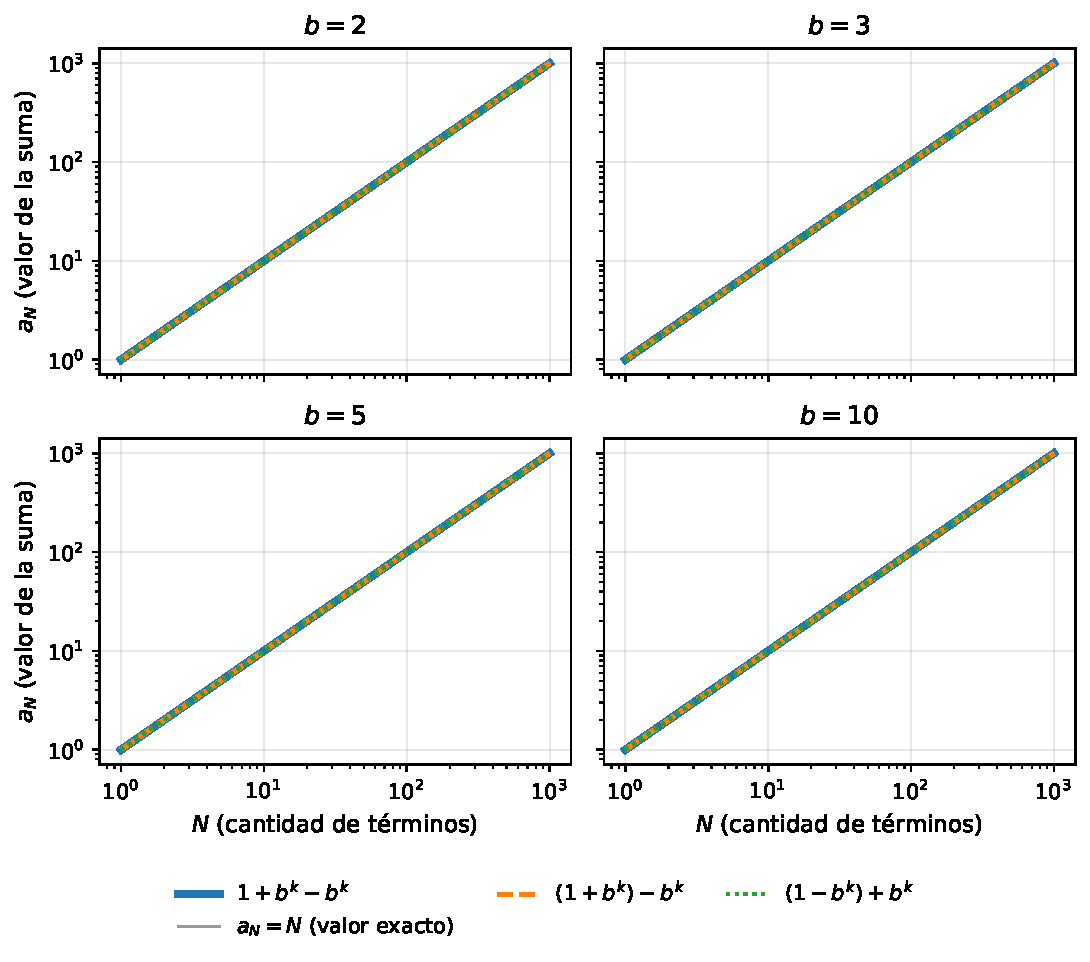
\includegraphics[width=\textwidth]{exp1-asociaciones-int.pdf}
  \caption{Valor de $a_N = \sum_{k=1}^{N} (1 + b^{k} - b^{k})$ para $N = 1, 2, \ldots, 1000$ con las
  tres asociaciones y $b$ de tipo \texttt{int}, en escala doblemente logarítmica. Cada panel
  corresponde a una base. La línea gris continua marca el valor exacto $a_N = N$. Las tres
  asociaciones coinciden con ella en todo el rango y por eso se superponen.}
  \label{fig:exp1-int}
\end{figure}

Con $b$ de tipo flotante el resultado cambia. La Figura \ref{fig:exp1-float} muestra que $a_N$
acompaña a $N$ solo hasta un valor $k^{\ast}$ que depende de la base y después se estanca en una
meseta. Más adelante la curva desaparece del gráfico: $a_N$ vale \texttt{NaN} a partir del primer
$k$ en que $b^{k}$ desborda a infinito. La Tabla \ref{tab:exp1-umbrales} reúne los tres números que
caracterizan cada base: el $k^{\ast}$ que predice la condición $b^{k} \ge 2^{53}$ de la sección
\ref{subsec:punto-flotante}, la altura de la meseta que alcanza cada asociación y el primer $k$ con
$b^{k} = \infty$. El $k^{\ast}$ predicho coincide con la meseta medida en todas las bases y
asociaciones salvo en $b = \pm 2.0$, donde alguna asociación difiere en un término. Las dos
primeras asociaciones dan resultados idénticos en las ocho bases de la tabla. La tercera se aparta
de las otras dos solo en $b = 2.0$, donde retiene un término más (53 contra 52), y en $b = -2.0$,
donde la asimetría se invierte.

\begin{figure}[htbp]
  \centering
  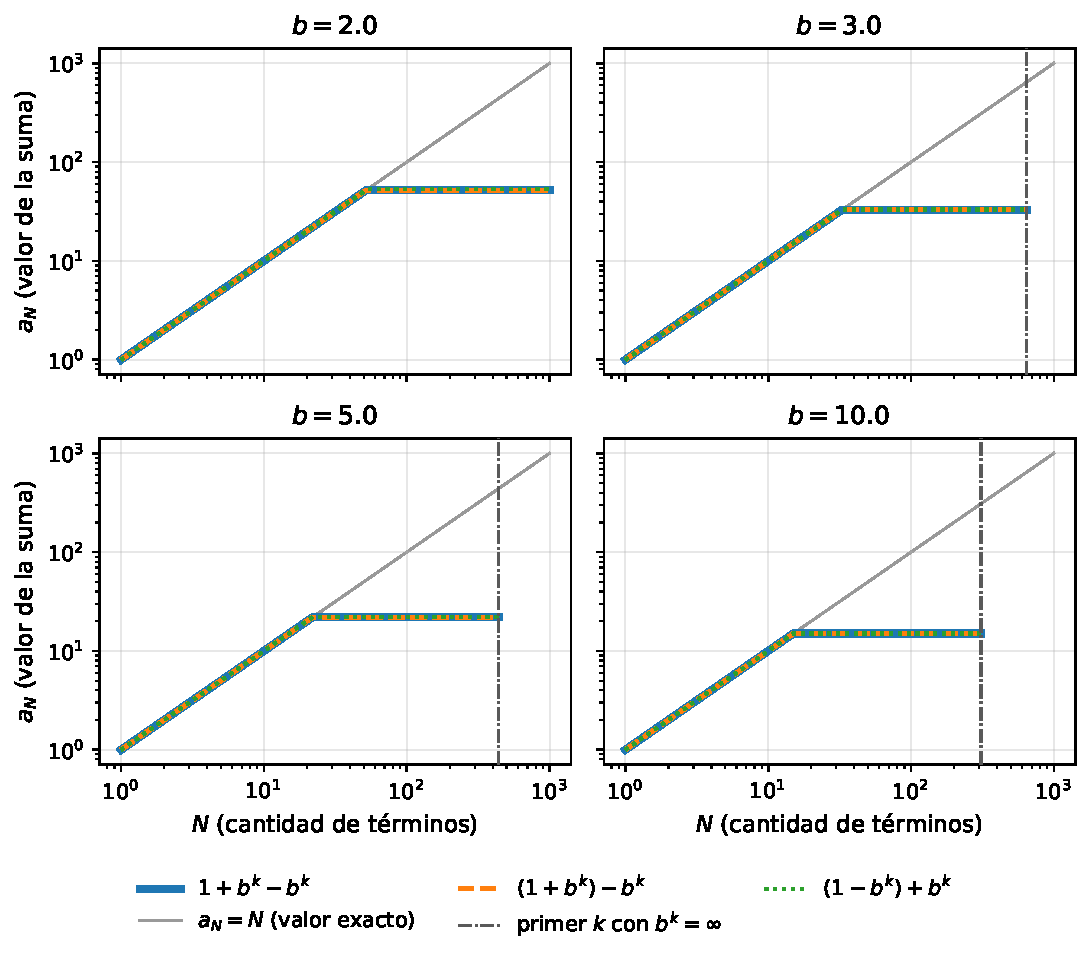
\includegraphics[width=\textwidth]{exp1-asociaciones-float.pdf}
  \caption{Valor de $a_N$ para $N = 1, 2, \ldots, 1000$ con las tres asociaciones y $b$ de tipo
  \texttt{float}, en escala doblemente logarítmica. La línea gris continua marca el valor exacto
  $a_N = N$ y la línea vertical de trazo y punto, el primer $k$ en que $b^{k}$ desborda a infinito.
  Las curvas se detienen ahí porque $a_N$ vale \texttt{NaN} de ese punto en adelante. Con
  $b = 2.0$ no hay desborde dentro del rango.}
  \label{fig:exp1-float}
\end{figure}

\begin{table}[htbp]
  \centering
  \caption{Umbrales medidos por base y asociación con $b$ de tipo \texttt{float}. La columna
  $k^{\ast}$ predicho es el mayor $k$ con $|b|^{k} < 2^{53}$; las tres siguientes son la altura de
  la meseta de $a_N$, es decir la cantidad de términos que aportan 1 antes de que el sumando se
  anule. La última columna indica el primer $k$ con $|b|^{k} = \infty$.}
  \label{tab:exp1-umbrales}
  \begin{tabular}{lrrrrr}
\toprule
$b$ & $k^\ast$ predicho & $1+b^k-b^k$ & $(1+b^k)-b^k$ & $(1-b^k)+b^k$ & $k$ con $b^k=\infty$ \\
\midrule
$2.0$ & $52$ & $52$ & $52$ & $53$ & sin desborde \\
$3.0$ & $33$ & $33$ & $33$ & $33$ & $647$ \\
$5.0$ & $22$ & $22$ & $22$ & $22$ & $442$ \\
$10.0$ & $15$ & $15$ & $15$ & $15$ & $309$ \\
$-2.0$ & $52$ & $53$ & $53$ & $52$ & sin desborde \\
$-3.0$ & $33$ & $33$ & $33$ & $33$ & $647$ \\
$-5.0$ & $22$ & $22$ & $22$ & $22$ & $442$ \\
$-10.0$ & $15$ & $15$ & $15$ & $15$ & $309$ \\
\bottomrule
\end{tabular}

\end{table}

El fenómeno no aparece cuando $0 \le b \le 1$. La Tabla \ref{tab:exp1-b-hasta-uno} cubre cinco
bases de ese rango, $b \in \{0.0,\, 0.1,\, 0.5,\, 0.9,\, 1.0\}$. El desvío de un término respecto de 1
nunca supera $1.11 \times 10^{-16}$, y el error final $|a_{1000} - 1000|$ es exactamente cero en
las cinco bases.
Con bases negativas, en cambio, se reproduce lo observado con las positivas. La Figura
\ref{fig:exp1-negativas} tiene la misma forma que la Figura \ref{fig:exp1-float}. Los umbrales de
las cuatro bases negativas de la Tabla \ref{tab:exp1-umbrales} coinciden con los de $|b|$ salvo la
inversión ya señalada en $b = \pm 2.0$.

\begin{table}[htbp]
  \centering
  \caption{Comportamiento con $0 \le b \le 1$. Las tres primeras columnas dan el desvío máximo de un
  término respecto de su valor exacto 1, para cada asociación y sobre $k = 1, \ldots, 1000$; la
  última, el error absoluto de la suma completa.}
  \label{tab:exp1-b-hasta-uno}
  \begin{tabular}{lrrrr}
\toprule
$b$ & $1+b^k-b^k$ & $(1+b^k)-b^k$ & $(1-b^k)+b^k$ & $|a_{1000} - 1000|$ \\
\midrule
$0.0$ & $0$ & $0$ & $0$ & $0$ \\
$0.1$ & $1.11 \times 10^{-16}$ & $1.11 \times 10^{-16}$ & $0$ & $0$ \\
$0.5$ & $1.11 \times 10^{-16}$ & $1.11 \times 10^{-16}$ & $0$ & $0$ \\
$0.9$ & $1.11 \times 10^{-16}$ & $1.11 \times 10^{-16}$ & $0$ & $0$ \\
$1.0$ & $0$ & $0$ & $0$ & $0$ \\
\bottomrule
\end{tabular}

\end{table}

\begin{figure}[htbp]
  \centering
  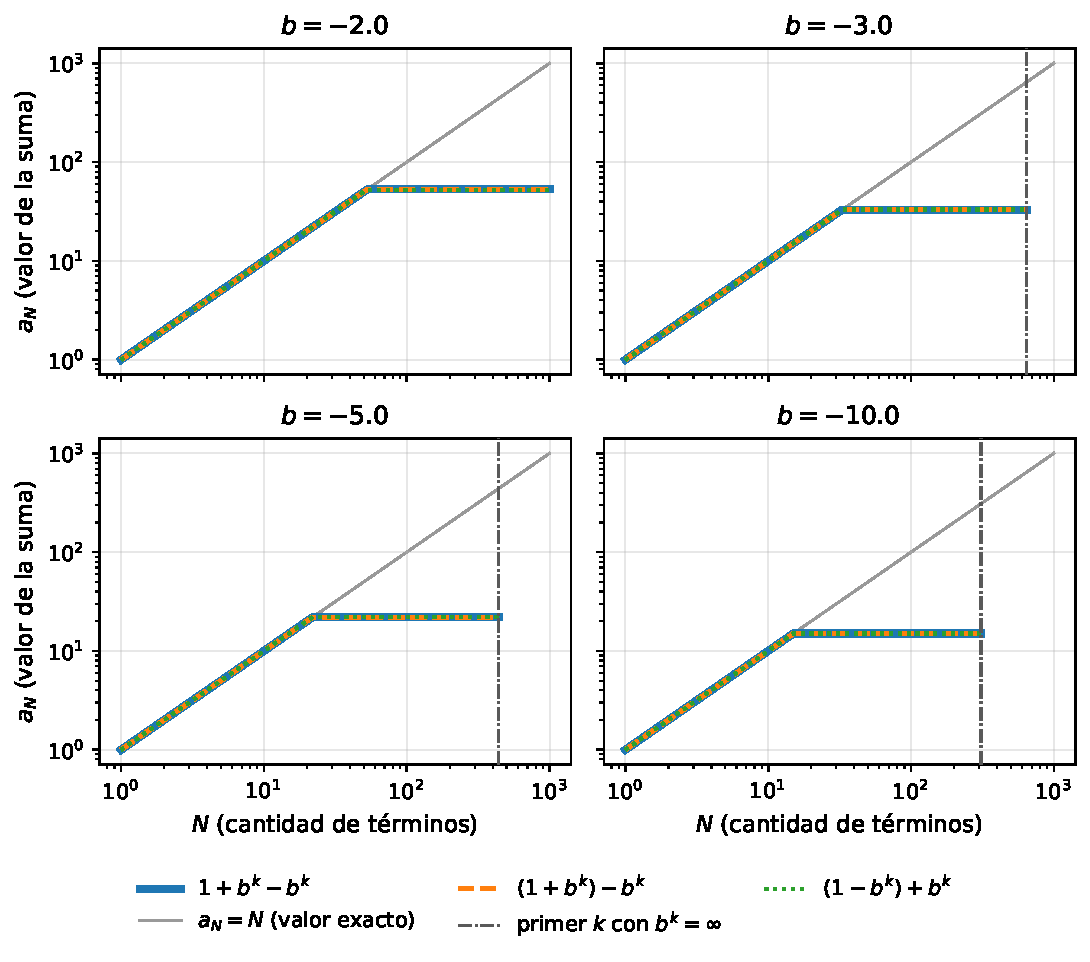
\includegraphics[width=\textwidth]{exp1-bases-negativas.pdf}
  \caption{Valor de $a_N$ para $N = 1, 2, \ldots, 1000$ con bases negativas de tipo \texttt{float},
  en escala doblemente logarítmica. Cada panel corresponde a una base. La línea gris continua marca
  el valor exacto $a_N = N$ y la línea vertical de trazo y punto, el primer $k$ en que $b^{k}$
  desborda a infinito; las curvas se detienen ahí porque $a_N$ vale \texttt{NaN} de ese punto en
  adelante. Con $b = -2.0$ no hay desborde dentro del rango.}
  \label{fig:exp1-negativas}
\end{figure}

Los enteros de ancho fijo dan un resultado distinto del de los flotantes. La Tabla
\ref{tab:exp1-int64} registra, para un entero con signo de 64 bits, el primer $k$ en que $b^{k}$
sale del rango representable, el valor exacto de esa potencia y el valor que efectivamente queda
almacenado, que en tres de las cuatro bases tiene el signo cambiado. Pese a eso, $a_{1000}$ vale
1000 en las cuatro bases, igual que con los enteros de Python.

\begin{table}[htbp]
  \centering
  \caption{Desborde de los enteros de 64 bits. Para cada base se indica el primer $k$ cuya potencia
  excede el rango de un entero con signo de 64 bits, el valor exacto de $b^{k}$, el valor
  almacenado tras el desborde y el resultado de la suma completa, calculado con la simulación de
  la aritmética de 64 bits y con el entero de precisión arbitraria de Python.}
  \label{tab:exp1-int64}
  \begin{tabular}{lrrrrr}
\toprule
$b$ & $k$ del desborde & $b^k$ exacto & $b^k$ en 64 bits & $a_{1000}$ (64 bits) & $a_{1000}$ (Python) \\
\midrule
$2$ & $63$ & $9.22 \times 10^{18}$ & $-9.22 \times 10^{18}$ & $1000$ & $1000$ \\
$3$ & $40$ & $1.22 \times 10^{19}$ & $-6.29 \times 10^{18}$ & $1000$ & $1000$ \\
$5$ & $28$ & $3.73 \times 10^{19}$ & $3.59 \times 10^{17}$ & $1000$ & $1000$ \\
$10$ & $19$ & $1.00 \times 10^{19}$ & $-8.45 \times 10^{18}$ & $1000$ & $1000$ \\
\bottomrule
\end{tabular}

\end{table}

El costo de la aritmética exacta se midió aparte. La Tabla \ref{tab:exp1-costo} muestra que el
tamaño de $b^{N}$ crece linealmente con $N$, hasta 332\,193 bits (43.3 KiB) en $N = 100\,000$,
mientras que el tiempo de la corrida con enteros crece más rápido que el de flotantes: el cociente
entre ambos crece con $N$ y llega a dos órdenes de magnitud en $N = 100\,000$.

\begin{table}[htbp]
  \centering
  \caption{Costo de los enteros de precisión arbitraria con $b = 10$. Se informa el tamaño de la
  última potencia calculada, en bits y en KiB, y el tiempo de la corrida completa con \texttt{int}
  y con \texttt{float}, en milisegundos.}
  \label{tab:exp1-costo}
  \begin{tabular}{lrrrrr}
\toprule
$N$ & bits de $b^N$ & memoria de $b^N$ (KiB) & $t$ con int (ms) & $t$ con float (ms) & cociente \\
\midrule
$1\,000$ & $3\,322$ & $0.5$ & $0.23$ & $0.05$ & $4$ \\
$5\,000$ & $16\,610$ & $2.2$ & $3.50$ & $0.25$ & $14$ \\
$10\,000$ & $33\,220$ & $4.4$ & $12.41$ & $0.51$ & $25$ \\
$20\,000$ & $66\,439$ & $8.7$ & $44.46$ & $1.01$ & $44$ \\
$50\,000$ & $166\,097$ & $21.7$ & $252.51$ & $2.66$ & $95$ \\
$100\,000$ & $332\,193$ & $43.3$ & $987.15$ & $5.21$ & $189$ \\
\bottomrule
\end{tabular}


  \vspace{0.5em}
  \begin{minipage}{0.92\textwidth}
    \small \textit{Nota.} Cada tiempo es el mínimo de tres repeticiones tomadas con
    \texttt{time.perf\_counter()} y depende de la máquina y de la carga del sistema, así que tanto
    los valores absolutos como su cociente cambian entre corridas.
  \end{minipage}
\end{table}

\subsection{Dependencia del orden de suma}
\label{subsec:res-orden}

Los cuatro algoritmos de suma aplicados a $b_N = \sum_{k=1}^{N} 1/(k(k+1))$ producen resultados
distintos entre sí, y la diferencia crece con $N$. La Figura \ref{fig:exp2-error} separa las cuatro
curvas en dos grupos. Acumular de mayor a menor módulo y acumular en orden aleatorio dan errores
relativos que crecen con $N$ y llegan al orden de $10^{-14}$ en el extremo del rango grande.
Acumular de menor a mayor módulo y la suma de Kahan se mantienen en el orden de $10^{-16}$ sobre
las dos grillas, sin tendencia creciente. La cota $\sqrt{N}\,u$ de la ecuación
\eqref{eq:cota-raiz}, dibujada en la misma figura, queda por encima de las dos curvas que crecen en
todo el rango.

\begin{figure}[htbp]
  \centering
  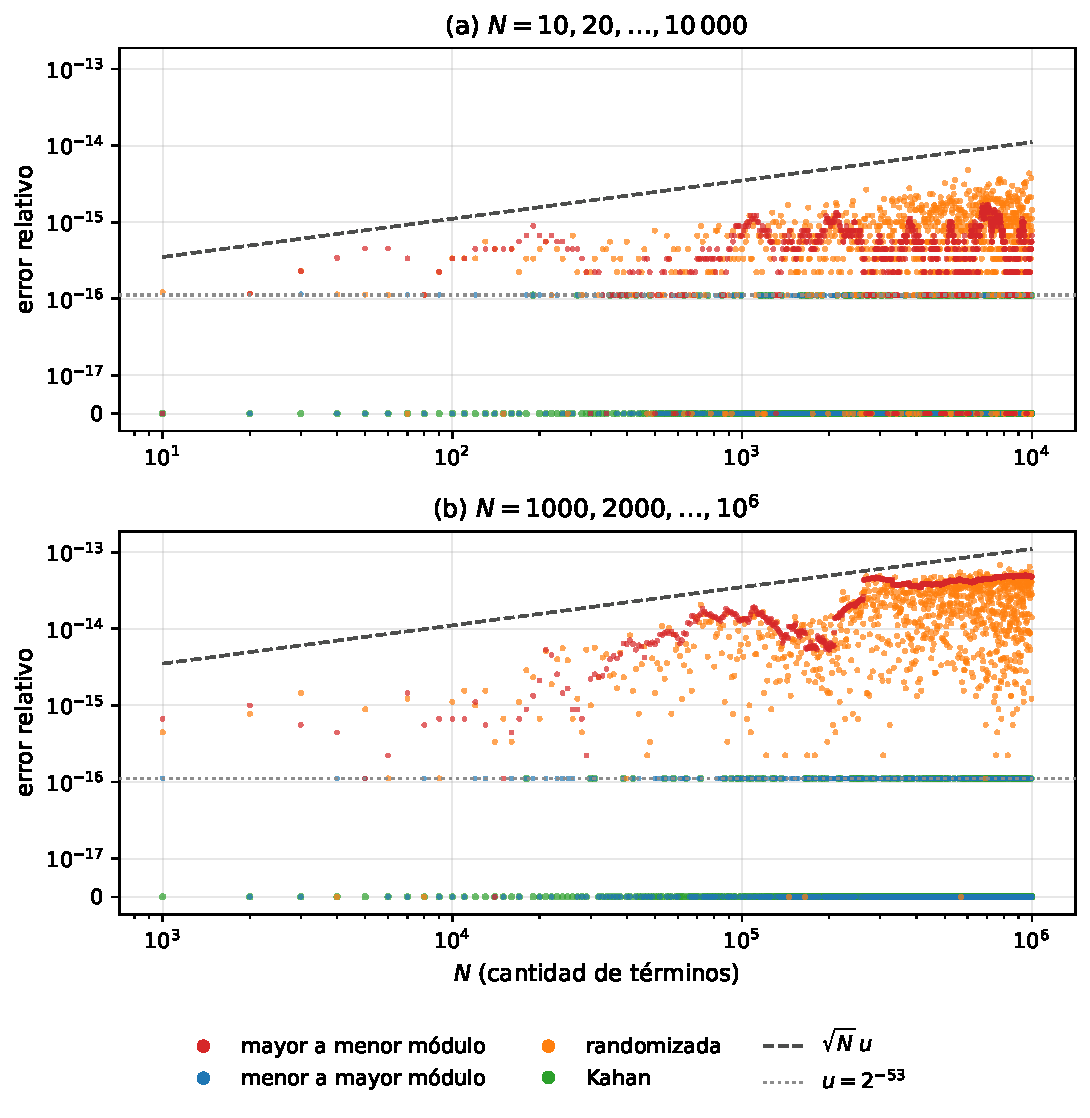
\includegraphics[width=\textwidth]{exp2-error-relativo.pdf}
  \caption{Error relativo de $b_N$ respecto de la forma cerrada $N/(N+1)$ para los cuatro
  algoritmos de suma, en escala \texttt{symlog} en el eje vertical, que permite mostrar los valores
  exactamente nulos junto con los positivos. El panel (a) cubre $N = 10, 20, \ldots, 10\,000$ y el
  panel (b), $N = 1000, 2000, \ldots, 10^{6}$. Las líneas grises marcan la cota estadística
  $\sqrt{N}\,u$ y la unidad de redondeo $u = 2^{-53}$. Se usan marcadores en lugar de líneas porque
  las curvas de menor a mayor y de Kahan se superponen casi por completo.}
  \label{fig:exp2-error}
\end{figure}

\begin{table}[htbp]
  \centering
  \caption{Error relativo de $b_N$ respecto de $N/(N+1)$ para los cuatro algoritmos, en seis
  valores de $N$ separados por un factor 10.}
  \label{tab:exp2-errores}
  \begin{tabular}{lrrrr}
\toprule
$N$ & mayor a menor & menor a mayor & randomizada & Kahan \\
\midrule
$10$ & $0$ & $0$ & $1.22 \times 10^{-16}$ & $0$ \\
$100$ & $3.36 \times 10^{-16}$ & $0$ & $3.36 \times 10^{-16}$ & $0$ \\
$1\,000$ & $6.67 \times 10^{-16}$ & $1.11 \times 10^{-16}$ & $4.45 \times 10^{-16}$ & $0$ \\
$10\,000$ & $6.66 \times 10^{-16}$ & $0$ & $1.11 \times 10^{-15}$ & $0$ \\
$100\,000$ & $1.31 \times 10^{-14}$ & $1.11 \times 10^{-16}$ & $1.34 \times 10^{-14}$ & $1.11 \times 10^{-16}$ \\
$1\,000\,000$ & $4.76 \times 10^{-14}$ & $0$ & $1.41 \times 10^{-14}$ & $0$ \\
\bottomrule
\end{tabular}

\end{table}

La Tabla \ref{tab:exp2-errores} da los valores puntuales en seis $N$ y la Tabla
\ref{tab:exp2-resumen} resume las dos grillas completas. Sobre los mil valores de $N$ del rango
grande, la suma de menor a mayor módulo y la de Kahan alcanzan el valor de referencia sin error
medible en 599 y 862 casos respectivamente, contra 1 caso de la suma de mayor a menor y 5 de la
randomizada. Los máximos de las dos primeras se mantienen entre $1.11$ y $1.15 \times 10^{-16}$, es
decir en el nivel de $u$, y no crecen al pasar de la grilla chica a la grande. Los de las otras dos
crecen un orden de magnitud entre una grilla y la otra.

\begin{table}[htbp]
  \centering
  \caption{Resumen de los cuatro algoritmos sobre las dos grillas completas, de mil valores de $N$
  cada una. Las dos primeras columnas dan el error relativo máximo en cada grilla y la última, en
  cuántos valores de $N$ de la grilla grande el resultado coincide bit a bit con la forma cerrada.}
  \label{tab:exp2-resumen}
  \begin{tabular}{lrrr}
\toprule
algoritmo & máximo, $N \leq 10^{4}$ & máximo, $N \leq 10^{6}$ & $N$ con $E_\mathrm{rel} = 0$ \\
\midrule
mayor a menor módulo & $1.67 \times 10^{-15}$ & $5.03 \times 10^{-14}$ & $1$ de $1000$ \\
menor a mayor módulo & $1.15 \times 10^{-16}$ & $1.11 \times 10^{-16}$ & $599$ de $1000$ \\
randomizada & $4.77 \times 10^{-15}$ & $6.84 \times 10^{-14}$ & $5$ de $1000$ \\
Kahan & $1.12 \times 10^{-16}$ & $1.11 \times 10^{-16}$ & $862$ de $1000$ \\
\bottomrule
\end{tabular}

\end{table}

Repetir la suma randomizada 50 veces con $N = 10^{6}$, cada vez con una permutación distinta,
produce 48 resultados diferentes: dos pares de repeticiones coinciden. La Figura
\ref{fig:exp2-dispersion} muestra la dispersión de esos errores junto con los valores de los
algoritmos deterministas, y la Tabla \ref{tab:exp2-dispersion} la resume. El error relativo va de
$2.22 \times 10^{-16}$ a $5.64 \times 10^{-14}$, con mediana $2.10 \times 10^{-14}$ y desvío
estándar $1.47 \times 10^{-14}$. El mayor supera al menor en un factor 254. Para el
mismo $N$, la suma de mayor a menor módulo da un error de $4.76 \times 10^{-14}$, por encima de la
mediana de la randomizada y por debajo de su máximo.

\begin{figure}[htbp]
  \centering
  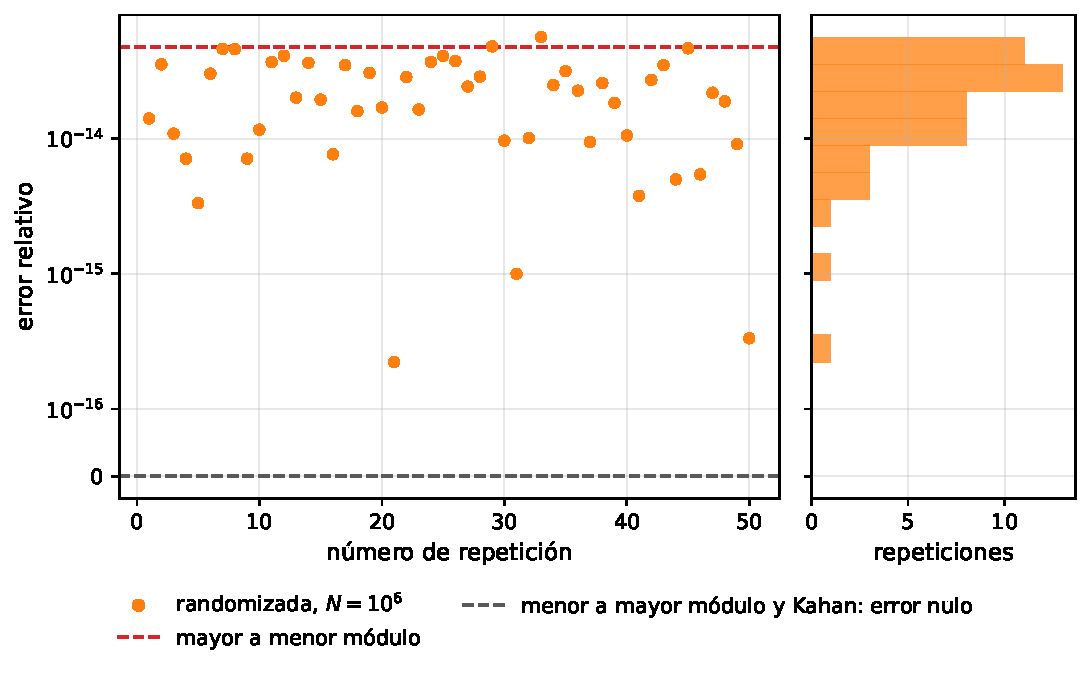
\includegraphics[width=\textwidth]{exp2-dispersion-randomizada.pdf}
  \caption{Dispersión de la suma randomizada con $N = 10^{6}$ sobre 50 repeticiones, cada una con
  una permutación distinta derivada de la semilla maestra. El panel izquierdo muestra el error
  relativo de cada repetición y el derecho, su histograma. Las dos líneas horizontales a trazos
  marcan los algoritmos deterministas para el mismo $N$: la de arriba, el error de la suma de mayor
  a menor módulo; la de abajo, el error nulo de las sumas de menor a mayor y de Kahan. El eje
  vertical usa escala \texttt{symlog}, que da lugar al valor nulo.}
  \label{fig:exp2-dispersion}
\end{figure}

\begin{table}[htbp]
  \centering
  \caption{Dispersión del error relativo de la suma randomizada sobre 50 repeticiones con
  $N = 10^{6}$.}
  \label{tab:exp2-dispersion}
  \begin{tabular}{lr}
\toprule
magnitud & valor \\
\midrule
repeticiones & $50$ \\
resultados $b_N$ distintos & $48$ \\
$E_\mathrm{rel}$ mínimo & $2.22 \times 10^{-16}$ \\
$E_\mathrm{rel}$ mediana & $2.10 \times 10^{-14}$ \\
$E_\mathrm{rel}$ máximo & $5.64 \times 10^{-14}$ \\
desvío estándar de $E_\mathrm{rel}$ & $1.47 \times 10^{-14}$ \\
cociente máximo sobre mínimo & $254$ \\
\bottomrule
\end{tabular}

\end{table}

\subsection{Representaciones equivalentes de una misma suma}
\label{subsec:res-representaciones}

Las dos representaciones de $b_N$, la suma de $1/(k(k+1))$ y la telescópica
$\sum (1/k - 1/(k+1))$, no producen el mismo flotante. Coinciden bit a bit en 1 de los 1001 valores
de $N$ de la grilla, únicamente en $N = 1$, y en el resto se separan por unas pocas unidades en el
último lugar, según la última columna de la Tabla \ref{tab:exp3-bn}. Ninguna de las dos se degrada
con $N$. La Figura \ref{fig:exp3-bn} muestra las dos curvas de error contenidas por la cota
$\sqrt{N}\,u$ y sin tendencia creciente. La Tabla \ref{tab:exp3-resumen} da máximos de
$1.67 \times 10^{-15}$ y $1.33 \times 10^{-15}$ sobre la grilla completa, con error exactamente
nulo en 68 y 97 valores de $N$ respectivamente.

\begin{figure}[htbp]
  \centering
  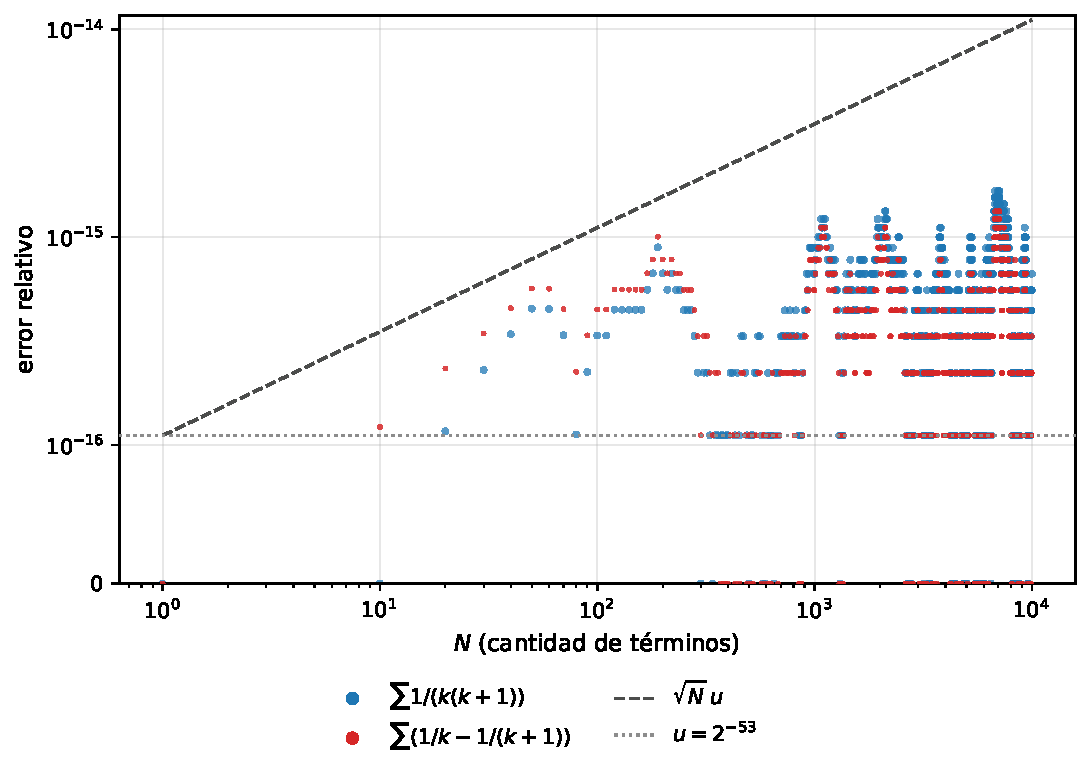
\includegraphics[width=\textwidth]{exp3-representaciones-bn.pdf}
  \caption{Error relativo de las dos representaciones de $b_N$ respecto de la forma cerrada
  $N/(N+1)$, para $N = 1, 10, 20, \ldots, 10\,000$, en escala \texttt{symlog} en el eje vertical
  para incluir los valores nulos. Las líneas grises marcan la cota estadística $\sqrt{N}\,u$ y la
  unidad de redondeo $u = 2^{-53}$.}
  \label{fig:exp3-bn}
\end{figure}

\begin{table}[htbp]
  \centering
  \caption{Error relativo de las dos representaciones de $b_N$ respecto de $N/(N+1)$ en cinco
  valores de $N$, con $b_N^{(1)} = \sum_k 1/(k(k+1))$ y $b_N^{(2)} = \sum_k (1/k - 1/(k+1))$. La
  última columna da la distancia entre los dos resultados medida en unidades del último lugar (ulp)
  del valor exacto.}
  \label{tab:exp3-bn}
  \begin{tabular}{lrrr}
\toprule
$N$ & $E_\mathrm{rel}$ de $b_N^{(1)}$ & $E_\mathrm{rel}$ de $b_N^{(2)}$ & $|b_N^{(1)} - b_N^{(2)}|$ (ulp) \\
\midrule
$1$ & $0$ & $0$ & $0$ \\
$10$ & $0$ & $1.22 \times 10^{-16}$ & $1$ \\
$100$ & $3.36 \times 10^{-16}$ & $4.49 \times 10^{-16}$ & $1$ \\
$1\,000$ & $6.67 \times 10^{-16}$ & $5.56 \times 10^{-16}$ & $1$ \\
$10\,000$ & $6.66 \times 10^{-16}$ & $3.33 \times 10^{-16}$ & $3$ \\
\bottomrule
\end{tabular}

\end{table}

\begin{table}[htbp]
  \centering
  \caption{Resumen de las dos sucesiones del tercer experimento sobre la grilla completa de 1001
  valores de $N$. Las cinco primeras filas corresponden a $b_N$, con
  $b_N^{(1)} = \sum_k 1/(k(k+1))$ y $b_N^{(2)} = \sum_k (1/k - 1/(k+1))$, medidas contra la forma
  cerrada $N/(N+1)$. La última fila corresponde a $c_N$, que no tiene forma cerrada: $D_N$ es la
  discrepancia absoluta entre sus dos representaciones y nunca se anula.}
  \label{tab:exp3-resumen}
  \begin{tabular}{lr}
\toprule
magnitud & valor \\
\midrule
$E_\mathrm{rel}$ máximo de $b_N^{(1)}$ & $1.67 \times 10^{-15}$ \\
$E_\mathrm{rel}$ máximo de $b_N^{(2)}$ & $1.33 \times 10^{-15}$ \\
$N$ con $E_\mathrm{rel} = 0$ en $b_N^{(1)}$ & $68$ de $1001$ \\
$N$ con $E_\mathrm{rel} = 0$ en $b_N^{(2)}$ & $97$ de $1001$ \\
$N$ con $b_N^{(1)} = b_N^{(2)}$ & $1$ de $1001$ \\
$N$ con $D_N = 0$ & $0$ de $1001$ \\
\bottomrule
\end{tabular}

\end{table}

La sucesión $c_N$ se comporta de otra manera. La discrepancia $D_N$ entre sus dos representaciones
no es nula en ninguno de los 1001 valores de $N$ y crece de $5.55 \times 10^{-17}$ en $N = 1$ a
$2.85 \times 10^{-11}$ en $N = 10\,000$, según la Tabla \ref{tab:exp3-cn}. En términos de cifras
significativas, los dos resultados comparten 15 en $N = 1$ y 11 en $N = 10\,000$. El panel (a) de la
Figura \ref{fig:exp3-cn} muestra esa curva junto con la suma de las discrepancias de los términos
individuales, que coincide con $D_N$ en $N = 1$, donde hay un solo término, y queda por encima en
todo el resto del rango. La misma figura incluye la cota $N^{2}u$ de la sección
\ref{subsec:cancelacion}, que acota a las dos.

\begin{table}[htbp]
  \centering
  \small
  \caption{Discrepancia entre las dos representaciones de $c_N$ en cinco valores de $N$. Se informa
  el valor calculado con la representación como cociente, la discrepancia absoluta
  $D_N = |c_N^{(1)} - c_N^{(2)}|$, su cociente con $c_N$ y la cantidad de cifras decimales
  significativas en que los dos resultados coinciden.}
  \label{tab:exp3-cn}
  \begin{tabular}{lrrrr}
\toprule
$N$ & $c_N^{(1)}$ & $D_N$ & $D_N/c_N^{(1)}$ & cifras coincidentes \\
\midrule
$1$ & $0.414213562373$ & $5.55 \times 10^{-17}$ & $1.34 \times 10^{-16}$ & $15$ \\
$10$ & $1.356033188972$ & $2.22 \times 10^{-16}$ & $1.64 \times 10^{-16}$ & $15$ \\
$100$ & $2.484679664884$ & $6.22 \times 10^{-15}$ & $2.50 \times 10^{-15}$ & $14$ \\
$1\,000$ & $3.633720211117$ & $1.79 \times 10^{-13}$ & $4.91 \times 10^{-14}$ & $13$ \\
$10\,000$ & $4.784787737052$ & $2.85 \times 10^{-11}$ & $5.95 \times 10^{-12}$ & $11$ \\
\bottomrule
\end{tabular}

\end{table}

Término a término, la discrepancia relativa entre $\sqrt{k^{2}+1} - k$ y $1/(\sqrt{k^{2}+1} + k)$
crece con $k$ conforme a la cota $2k^{2}u$ de la ecuación \eqref{eq:cota-termino}, como muestra el
panel (b) de la Figura \ref{fig:exp3-cn}. La Tabla \ref{tab:exp3-terminos} compara el $k$ que
predice esa cota con el primero que efectivamente cruza cada umbral: la discrepancia supera
$10^{-12}$ en $k = 87$, $10^{-8}$ en $k = 8193$ y $10^{-6}$ en $k = 68\,985$, entre 1.03 y 1.33
veces el valor predicho. En el último umbral la coincidencia es exacta: la cota sitúa el colapso
completo en $k = 2^{26} = 67\,108\,864$ y ese es el primer $k$ en que $\sqrt{k^{2}+1}$ devuelve
exactamente $k$. Ahí el término calculado como diferencia vale cero y el calculado como cociente
sigue siendo positivo.

\begin{figure}[htbp]
  \centering
  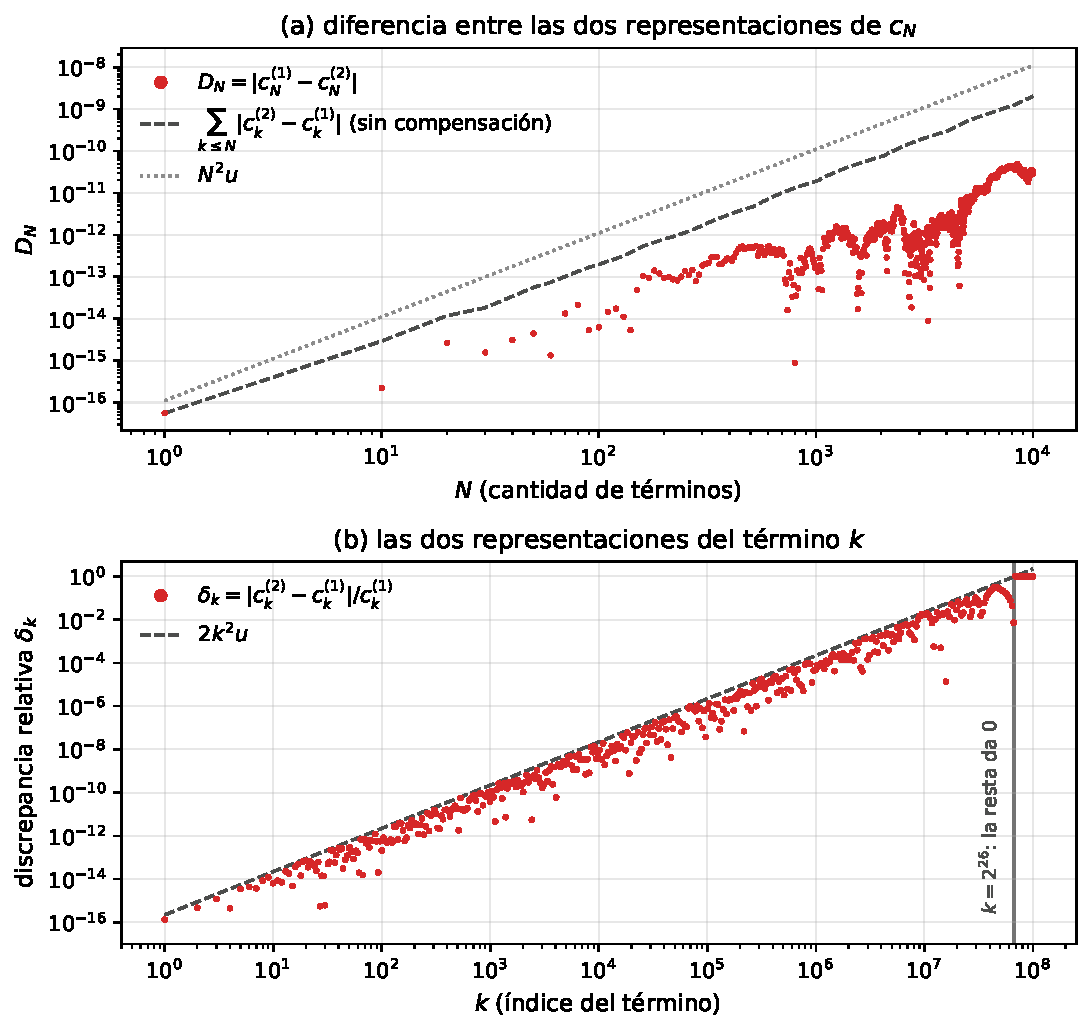
\includegraphics[width=\textwidth]{exp3-cancelacion-cn.pdf}
  \caption{Cancelación en $c_N$, con $c_N^{(1)} = \sum_k 1/(\sqrt{k^{2}+1} + k)$ la representación
  como cociente y $c_N^{(2)} = \sum_k (\sqrt{k^{2}+1} - k)$ la representación como diferencia. El
  panel (a) muestra la discrepancia absoluta
  $D_N = |c_N^{(1)} - c_N^{(2)}|$ entre las dos representaciones para
  $N = 1, 10, 20, \ldots, 10\,000$, junto con la suma de las discrepancias de los términos, que es
  lo que valdría $D_N$ si los errores de cada término no se compensaran entre sí, y con la cota
  $N^{2}u$. El panel (b) muestra la discrepancia relativa $\delta_k$ entre las dos formas del
  término $k$ sobre una grilla logarítmica hasta $k = 10^{8}$, con la cota $2k^{2}u$ y con el
  primer $k$ en que la resta devuelve cero. Los dos paneles usan escala logarítmica en los dos
  ejes.}
  \label{fig:exp3-cn}
\end{figure}

\begin{table}[htbp]
  \centering
  \caption{Umbrales de la discrepancia relativa $\delta_k$ entre las dos representaciones del término $k$ de
  $c_N$. Para cada umbral $\varepsilon$ se compara el $k$ que predice la cota $2k^{2}u$ con el
  primer $k$ medido que alcanza ese umbral.}
  \label{tab:exp3-terminos}
  \begin{tabular}{lrrr}
\toprule
$\varepsilon$ & $k$ que predice $2k^{2}u$ & primer $k$ con $\delta_k \ge \varepsilon$ & $\delta_k$ en ese $k$ \\
\midrule
$1 \times 10^{-12}$ & $68$ & $87$ & $1.21 \times 10^{-12}$ \\
$1 \times 10^{-10}$ & $672$ & $895$ & $1.01 \times 10^{-10}$ \\
$1 \times 10^{-8}$ & $6\,711$ & $8\,193$ & $1.12 \times 10^{-8}$ \\
$1 \times 10^{-6}$ & $67\,109$ & $68\,985$ & $1.00 \times 10^{-6}$ \\
$1$ & $67\,108\,864$ & $67\,108\,864$ & $1$ \\
\bottomrule
\end{tabular}

\end{table}

Las dos formas cerradas de $b_N$, en cambio, casi siempre coinciden. La Tabla
\ref{tab:exp3-cerradas} muestra que $1 - 1/(N+1)$ y $N/(N+1)$ difieren en 4 de los 1001 valores de
$N$ de la grilla y en 19 de los primeros 99\,999, siempre por exactamente 1 ulp. Medidos contra el
valor racional exacto, el error relativo máximo es $1.11 \times 10^{-16}$ para la primera forma y
$5.55 \times 10^{-17}$ para la segunda, es decir la mitad. Las dos saturan en 1 alrededor de
$N = 1.8 \times 10^{16}$, con un valor de $N$ de diferencia entre una y otra.

\begin{table}[htbp]
  \centering
  \caption{Comparación de las dos formas cerradas de $b_N$. Las discrepancias se cuentan sobre la
  grilla del experimento y sobre todos los $N$ menores que $100\,000$; los errores relativos se
  miden contra el valor racional exacto calculado con aritmética de fracciones. Las dos últimas
  filas dan el primer $N$ en que cada forma devuelve exactamente 1.}
  \label{tab:exp3-cerradas}
  \begin{tabular}{lr}
\toprule
magnitud & valor \\
\midrule
$N$ de la grilla donde difieren & $4$ de $1001$ \\
cuáles son esos $N$ & $170$, $510$, $1\,970$, $3\,590$ \\
$N <$ $100\,000$ donde difieren & $19$ de $99\,999$ \\
separación cuando difieren & $1$ ulp \\
$E_\mathrm{rel}$ máximo de $1 - 1/(N+1)$ & $1.11 \times 10^{-16}$ \\
$E_\mathrm{rel}$ máximo de $N/(N+1)$ & $5.55 \times 10^{-17}$ \\
primer $N$ con $1 - 1/(N+1) = 1$ & $18\,014\,398\,509\,481\,982$ \\
primer $N$ con $N/(N+1) = 1$ & $18\,014\,398\,509\,481\,983$ \\
\bottomrule
\end{tabular}

\end{table}

\section{Discusión}
\label{sec:discusion}
% Interpretación, comparación con la teoría, hallazgos inesperados, limitaciones.
% Organizado por los mismos tres fenómenos que Resultados.

\subsection{Pérdida de la asociatividad}
\label{subsec:dis-asociatividad}

El contraste entre las Figuras \ref{fig:exp1-int} y \ref{fig:exp1-float} separa dos aritméticas que
la notación matemática no distingue. Con $b$ de tipo \texttt{int}, la identidad $1 + b^{k} - b^{k} = 1$
se traslada al programa sin pérdida porque el entero de Python es exacto y no tiene techo
(sección \ref{subsec:enteros}); las tres asociaciones son entonces tres formas de escribir el mismo
cálculo. Con $b$ de tipo \texttt{float} la identidad deja de valer en cuanto $b^{k}$ alcanza el
tamaño en que el 1 ya no cabe en la mantisa del acumulador. La coincidencia entre el $k^{\ast}$
predicho por la condición $b^{k} \ge 2^{53}$ y la altura de la meseta medida, exacta en seis de las
ocho bases de la Tabla \ref{tab:exp1-umbrales} y con un término de diferencia en las dos restantes,
indica que el efecto no depende de detalles de la implementación
sino del espaciado de $\mathbb{F}$ descrito en \eqref{eq:binary64}. Es el contraejemplo
\eqref{eq:contraejemplo} repetido a lo largo de un barrido.

Conviene precisar qué falla. La potencia $b^{k}$ está bien calculada dentro de lo que el formato
permite; lo que se pierde es el 1, absorbido en la suma $1 + b^{k}$. El término no se anula porque
$b^{k}$ sea inexacto, sino porque la agrupación decide en qué momento el 1 se encuentra con un
número demasiado grande.

Las dos primeras asociaciones dieron resultados idénticos en todas las bases ensayadas, y la razón
es sintáctica antes que numérica: Python evalúa $1 + b^{k} - b^{k}$ de izquierda a derecha, así que
esa expresión y $(1 + b^{k}) - b^{k}$ describen la misma secuencia de operaciones. La consigna pide
comparar tres asociaciones y el lenguaje entrega dos programas distintos. El par idéntico deja
aislado el efecto del agrupamiento: las dos expresiones que se traducen a la misma secuencia
coinciden en todas las bases, y la única que se aparta es la que agrupa distinto.

La tercera asociación se aparta de las otras dos solo en $b = \pm 2.0$, y ahí difiere en un
término: retiene uno más con $b = 2.0$ y uno menos con $b = -2.0$. El mecanismo es la asimetría entre binadas vecinas señalada en la sección
\ref{subsec:punto-flotante}: en $[2^{52}, 2^{53})$ el espaciado vale 1 y en $[2^{53}, 2^{54})$ vale
2, de modo que $1 - 2^{53}$ es representable y $1 + 2^{53}$ no lo es. Restar primero deja el
resultado en la binada de abajo, que tiene el doble de resolución. Que el efecto aparezca
únicamente con $b = \pm 2$ es consecuencia de que solo esa base pisa exactamente el borde $2^{53}$:
con $b = 3$, $5$ o $10$ la potencia salta por encima del borde y las tres asociaciones pierden el
término en el mismo $k$. No alcanza con que la base sea potencia de dos. Con $b = 4$ las potencias
recorren los exponentes pares y saltan de $2^{52}$ a $2^{54}$ sin tocar $2^{53}$, de modo que las
tres asociaciones vuelven a coincidir. La inversión con $b = -2.0$ es la misma asimetría con los
signos cambiados.

Ese mecanismo también da cuenta del régimen $0 \le b \le 1$ de la Tabla
\ref{tab:exp1-b-hasta-uno}. El
fenómeno principal no aparece porque $|b|^{k}$ queda acotado por 1 y nunca se acerca a $2^{53}$; lo
que queda es el redondeo de $1 + b^{k}$, de medio ulp en la binada $[1, 2)$, es decir,
$2^{-53} = 1.11 \times 10^{-16}$, exactamente el valor máximo que registra la tabla para las dos
primeras asociaciones. La tercera, que resta primero y trabaja en la binada de abajo, no muestra
desvío en ninguna de las cinco bases. Que el error de la suma completa sea nulo pese a esos desvíos
es consistente con el mismo espaciado: el acumulador crece hasta 1000, donde el espaciado de
$\mathbb{F}$ vale $2^{-43} \approx 1.14 \times 10^{-13}$. Un desvío de $10^{-16}$ por término cae
por debajo de medio espaciado apenas el acumulador supera unas pocas unidades. El redondeo de la
acumulación descarta el error del término. El mismo mecanismo de absorción que arruina el
experimento con bases grandes lo salva con bases chicas.

El desborde a $\infty$ merece una lectura aparte. Cuando $b^{k}$ excede el mayor representable, el
estándar no interrumpe el cálculo: devuelve $\infty$, y la resta $\infty - \infty$ produce
\texttt{NaN}, que se propaga por el resto de la acumulación. Por eso las curvas de la Figura
\ref{fig:exp1-float} no se desvían: desaparecen. En términos prácticos, el desborde no se manifiesta
como una falla sino como un valor que contamina todo lo que viene después. Detectarlo exige
inspeccionar el resultado; el programa termina igual.

El comportamiento de los enteros de ancho fijo fue el primero de los dos resultados que
contradijeron la expectativa inicial. La
Tabla \ref{tab:exp1-int64} muestra que $b^{k}$ sale del rango de \texttt{int64} muy temprano, en
$k = 19$ para $b = 10$, y que el valor almacenado tiene el signo cambiado en tres de las cuatro
bases. Aun así $a_{1000}$ vale 1000 en las cuatro. La explicación está en la sección
\ref{subsec:enteros}: el entero de 64 bits reduce módulo $2^{64}$ en complemento a dos, y esa
aritmética es la de
un anillo, donde $(1 + x) - x = 1$ vale para todo $x$ sin excepción. El desborde entero no destruye
información, la reduce módulo $2^{64}$, y la resta posterior deshace la reducción. El redondeo de
punto flotante, en cambio, descarta bits de forma irreversible. Esa es la diferencia entre las dos
formas de perder magnitud, y es lo que hace que el mismo experimento revele el problema con
\texttt{float} y lo esconda con \texttt{int64}.

La conclusión que no se sigue de ese dato es que los enteros de ancho fijo sean seguros. La suma que
propone la consigna es justamente una en la que el valor desbordado se cancela contra sí mismo.
Cualquier expresión que use $b^{k}$ sin cancelarlo, por ejemplo una comparación, una división o una
impresión, entrega el valor de la cuarta columna de la Tabla \ref{tab:exp1-int64} y no el de la
tercera. A eso se suma que en C el desborde de un entero con signo es comportamiento indefinido
(ISO, 2018): el mismo programa ni siquiera tiene garantizado el resultado modular que sí produce
NumPy.

La aritmética exacta de Python resuelve el problema pero lo cobra. La Tabla \ref{tab:exp1-costo}
muestra que el tamaño de $b^{N}$ crece linealmente y el tiempo de la corrida completa, de manera
cuadrática, con un cociente contra la corrida en flotantes que crece hasta dos órdenes de magnitud
al ir de $N = 1000$ a $N = 100\,000$. El crecimiento coincide con el argumento de la sección \ref{subsec:enteros}: cada
multiplicación cuesta un tiempo proporcional a la longitud del operando y las longitudes crecen con
$k$. Para $N$ del orden de mil el sobrecosto es tolerable; para $N$ del orden de $10^{5}$, un solo
número ocupa 43.3 KiB y la corrida se vuelve dos órdenes de magnitud más lenta. La elección entre
exactitud y costo depende del tamaño del problema.

\subsection{Dependencia del orden de suma}
\label{subsec:dis-orden}

El primer punto es de nombre. El experimento se plantea sobre la propiedad conmutativa, pero lo que
los datos ponen a prueba es la asociatividad. La suma de punto flotante sí es conmutativa, porque
$\mathrm{fl}(x + y)$ depende del valor exacto de $x + y$ y de una función de redondeo simétrica en
sus argumentos. Los cuatro algoritmos de la Figura \ref{fig:exp2-error} suman exactamente los mismos
números y difieren solo en cómo encadenan las sumas parciales, es decir, en el agrupamiento. La
distinción se enunció en la sección \ref{subsec:asociatividad} y los resultados la sostienen: si el
efecto viniera de la conmutatividad, permutar los índices no debería cambiar nada, y cambia.

La separación de las cuatro curvas en dos grupos sigue lo que predice el análisis de la sección
\ref{subsec:asociatividad}. Los términos $1/(k(k+1))$ decrecen como $k^{-2}$, así que sumar de mayor
a menor lleva el acumulador cerca de 1 en las primeras iteraciones y obliga a los términos tardíos,
de orden $10^{-12}$ en $N = 10^{6}$, a competir con un espaciado local del orden de $10^{-16}$. Cada
uno pierde su parte baja. Sumar de menor a mayor agrupa primero los términos chicos entre sí, donde
el espaciado local es comparable a su tamaño, y esa información sobrevive hasta el final. La suma de
Kahan llega al mismo lugar por otro camino: recupera el residuo de cada redondeo y lo reinyecta, con la cota
$2u + O(Nu^{2})$ de la sección \ref{subsec:kahan}, que no crece con $N$. La Tabla
\ref{tab:exp2-resumen} lo confirma: los máximos de esos dos algoritmos quedan entre
$1.11$ y $1.15 \times 10^{-16}$, es decir, en el nivel de $u$, y no crecen al multiplicar $N$ por
cien.

De ahí sale la lectura práctica, que no es la esperable. Ordenar de menor a mayor módulo alcanza
para igualar a Kahan en esta serie: máximos indistinguibles, los dos al nivel de $u$, y la
diferencia queda en
la cantidad de $N$ con coincidencia bit a bit, 599 contra 862 de mil. Cuando el problema es el
orden, ordenar ya lo resuelve, y Kahan cuesta cuatro operaciones de punto flotante por término en
lugar de una. La ventaja de Kahan aparece cuando el orden no está disponible de antemano: acá los
términos vienen ordenados por construcción y basta recorrer el índice al revés. En una serie cuyas
magnitudes no se conocen sin calcularlas, ordenar exige una pasada previa y memoria para
guardar los términos. Kahan no necesita ninguna de las dos cosas.

Las dos curvas que crecen quedan contenidas por $\sqrt{N}\,u$ de \eqref{eq:cota-raiz} en todo el
rango, lo que respalda el modelo de errores independientes de media nula frente al análisis de peor
caso. La cota conservadora $Nu$ vale $1.11 \times 10^{-10}$ en $N = 10^{6}$ y el error medido es
$5.03 \times 10^{-14}$: sobreestima por más de tres órdenes de magnitud. Suponer que los $N-1$
redondeos se alinean en la misma dirección describe un caso posible y no el caso típico.

La Figura \ref{fig:exp2-error} muestra además una estructura que la teoría anticipa: los errores no
nulos se acomodan en bandas horizontales discretas y no en una nube continua. Como $b_N$ está cerca
de 1, la diferencia entre el resultado y la referencia solo puede tomar valores múltiplos del
espaciado local de $\mathbb{F}$. Lo que se ve en el eje vertical son
cantidades enteras de ulp.

La dispersión de la suma randomizada responde la pregunta de la consigna y agrega un matiz. La
respuesta es que no da siempre lo mismo: 48 resultados distintos en 50 repeticiones, con un error
que va de $2.22 \times 10^{-16}$ a $5.64 \times 10^{-14}$, un factor 254 entre el mejor y el peor
caso, según la Tabla \ref{tab:exp2-dispersion}. Las dos coincidencias no contradicen el resto. Los
resultados posibles son múltiplos discretos de un ulp dentro de un rango acotado, así que con 50
muestras las repeticiones son esperables. La variabilidad tampoco es aleatoriedad del hardware: cada
permutación define un agrupamiento distinto y el resultado de cada uno es determinista, tanto que
fijar la semilla reproduce las 50 corridas.

La comparación con el orden decreciente pide cuidado en las dos direcciones. En mediana la
randomizada es mejor, $2.10 \times 10^{-14}$ contra $4.76 \times 10^{-14}$ para el mismo $N$, porque
mezclar rompe el patrón sistemático de absorción que produce recorrer los términos de mayor a menor.
Pero su máximo sobre la grilla grande es peor, $6.84 \times 10^{-14}$ contra
$5.03 \times 10^{-14}$. El orden decreciente es impreciso y predecible; el aleatorio es en mediana
algo más preciso y no reproducible sin fijar la semilla. Para un cálculo que debe dar el mismo valor dos
veces, la segunda propiedad pesa más que la primera.

\subsection{Representaciones equivalentes de una misma suma}
\label{subsec:dis-representaciones}

Las dos sucesiones de este experimento responden de manera opuesta a la misma transformación
algebraica, y esa oposición es lo que explica cuándo la cancelación importa.

Para $b_N$, las dos representaciones no producen el mismo flotante, cosa que era previsible porque
describen programas distintos según la sección \ref{subsec:telescopicas}, pero ninguna se degrada.
La representación telescópica resta $1/k - 1/(k+1)$, dos cantidades cuyo cociente tiende a 1, de modo que la
cancelación se agrava con $k$; y sin embargo la Figura \ref{fig:exp3-bn} muestra las dos curvas
contenidas por $\sqrt{N}\,u$ y sin tendencia creciente. La razón es que el término completo es de
orden $k^{-2}$ y se suma contra un acumulador que tiende a 1. Las cifras que la resta arruina son
cifras bajas de un sumando pequeño, y la acumulación las iba a descartar de todos modos. La
cancelación es un problema cuando el término cancelado domina el resultado, no cuando es una
corrección menor. La ventaja de la representación telescópica en la Tabla \ref{tab:exp3-resumen}, 97 contra
68 valores de $N$ con error nulo y un máximo algo menor, es de unos pocos ulp y no muestra tendencia
con $N$; no alcanza para preferir una representación sobre la otra.

Para $c_N$ el resultado es el contrario: $D_N$ no se anula en ninguno de los 1001 valores de $N$ y
crece casi seis órdenes de magnitud sobre la grilla, hasta $2.85 \times 10^{-11}$. Las dos
representaciones pasan de coincidir en 15 cifras a coincidir en 11. Acá el término cancelado es el
resultado mismo. El mecanismo es el descrito en la sección \ref{subsec:cancelacion} y merece
enunciarse al revés de como sugiere el nombre del fenómeno: por el lema de Sterbenz la resta
$\sqrt{k^{2}+1} - k$ es exacta, y el error lo aporta el redondeo previo de la raíz, de tamaño
absoluto del orden de $ku$, que la resta deja al frente de un resultado de tamaño $1/(2k)$. La
cancelación catastrófica no crea error, expone el que los operandos ya traían.

El acuerdo entre esa derivación y las mediciones es el resultado más ajustado del trabajo. La cota
$2k^{2}u$ de \eqref{eq:cota-termino} se obtuvo con aproximaciones de primer orden, y la Tabla
\ref{tab:exp3-terminos} muestra que los umbrales medidos caen entre 1.03 y 1.33 veces los
predichos, siempre del lado conservador. En el umbral final la coincidencia deja de ser aproximada:
la cota sitúa la pérdida completa de cifras significativas en $k = 1/\sqrt{2u} = 2^{26}$ y el primer
$k$ en que $\sqrt{k^{2}+1}$ devuelve exactamente $k$ es $67\,108\,864 = 2^{26}$. Un argumento de
orden de magnitud acierta un umbral de ocho cifras.

Dos advertencias sobre cómo leer esos datos. La primera es que $D_N$ mide la discrepancia entre dos
cálculos y no el error de ninguno de los dos, porque $c_N$ no tiene forma cerrada contra la cual
comparar (sección \ref{subsec:error-relativo}). Atribuir casi todo $D_N$ a la representación por
diferencia es razonable: la representación como cociente suma en el denominador y su error
relativo por término se mantiene del orden de $u$. Aun así, es una atribución apoyada en la teoría
y no una medición directa. La segunda es que $D_N$ queda muy por debajo de la suma de las
discrepancias de los términos individuales, que aparece en el panel (a) de la Figura
\ref{fig:exp3-cn}. Los errores de los términos tienen signos distintos y se compensan parcialmente, el mismo
comportamiento de paseo aleatorio que sostiene \eqref{eq:cota-raiz}. La suma de las cotas describe
el caso en que todos los errores se alinean, y presentarla como el error esperado sería tan
pesimista como usar $Nu$ para la suma acumulada.

Las dos formas cerradas de $b_N$ dieron el segundo resultado contraintuitivo. Por conteo de
operaciones, $1 - 1/(N+1)$ acumula dos redondeos y $N/(N+1)$ uno solo, así que \eqref{eq:modelo}
predice para la primera una cota del doble. Los errores máximos contra el valor racional exacto de
la Tabla \ref{tab:exp3-cerradas} confirman esa relación con precisión: $1.11 \times 10^{-16}$
contra $5.55 \times 10^{-17}$. Lo que no se sigue de ahí es que las dos expresiones den resultados
distintos en la práctica. Difieren en 4 de los 1001 valores de la grilla y en 19 de los primeros
$99\,999$, siempre por exactamente 1 ulp, y saturan en 1 con un solo $N$ de diferencia entre una y
otra. El redondeo adicional casi nunca llega a cambiar el flotante devuelto: para que lo cambie, el
valor exacto tiene que caer lo bastante cerca del punto medio entre dos representables, y eso ocurre
en una fracción pequeña de los casos.

De la comparación entre $c_N$ y las formas cerradas sale el punto general del experimento. Contar
operaciones acota el error pero no lo predice caso por caso: dos expresiones con cotas que difieren
en un factor 2 pueden devolver el mismo flotante casi siempre, mientras que dos expresiones con
cotas que difieren en un factor $k^{2}$ terminan sin ninguna cifra en común. La recomendación de
Goldberg (1991) de preferir la forma que evita restar cantidades próximas queda respaldada de manera
asimétrica: elegirla no empeoró ningún caso de este trabajo, y en el término de $c_N$ es, hacia
$k = 2^{26}$, la diferencia entre un error relativo del orden de $u$ y la pérdida completa de las
cifras significativas.

\subsection{Limitaciones}
\label{subsec:limitaciones}

El alcance de estas conclusiones está acotado por cuatro decisiones de diseño.

La referencia contra la cual se mide es, en la mayoría de los casos, un flotante. El error relativo
de \eqref{eq:error-relativo} se calcula contra $N/(N+1)$ evaluado en \texttt{binary64}, de modo que
el piso de lo medible es del orden de $u$ y los ceros de las Tablas \ref{tab:exp2-resumen} y
\ref{tab:exp3-resumen} significan coincidencia bit a bit con esa referencia, no exactitud. Solo la
comparación de las formas cerradas usa un patrón exacto, calculado con aritmética de fracciones. Un
trabajo posterior podría repetir las grillas grandes contra un valor de referencia en precisión
extendida y separar el error del algoritmo del error de la referencia.

Todas las mediciones corresponden a un único formato, \texttt{binary64}, sobre una máquina y un
intérprete. Los umbrales dependen del formato de manera predecible: en \texttt{binary32} el techo
$2^{53}$ del primer experimento pasaría a $2^{24}$ y el colapso de $c_N$ se adelantaría en más de
cuatro órdenes de magnitud en $k$. Eso es una extrapolación de las fórmulas y no una medición. Los
tiempos de la Tabla \ref{tab:exp1-costo} son los más sensibles al entorno: solo el cociente entre
las dos columnas es una magnitud estable entre corridas.

Las tres sucesiones estudiadas tienen términos positivos y decrecientes, y las conclusiones sobre el
orden de suma no se trasladan más allá de esa clase. En una serie con términos de signos alternados,
la cancelación entre términos domina el balance de error y acumular de menor a mayor módulo puede
dejar las cancelaciones grandes para el final, es decir, empeorar el resultado. La ventaja de
ordenar que se observa acá depende de que todos los términos empujen en la misma dirección.

Los rangos también acotan lo que se puede afirmar. El estudio de dispersión usa 50 repeticiones, que
alcanzan para el rango, la mediana y el desvío, pero no para describir las colas de la distribución.
Las grillas llegan a $N = 10^{6}$ para las sumas y a $k = 10^{8}$ para los términos de $c_N$; la
concordancia con $\sqrt{N}\,u$ está verificada dentro de esos límites y extrapolarla a tamaños
mucho mayores, donde el término $O(Nu^{2})$ de la cota de Kahan deja de ser despreciable, no está
respaldado por estos datos.

\section{Conclusiones}
\label{sec:conclusiones}
% Síntesis, respuesta a los objetivos, recomendaciones, líneas futuras. Sin resultados nuevos.

Los tres experimentos responden al objetivo general con un mismo criterio. Las propiedades
algebraicas de la suma dejan de valer en la computadora cuando la magnitud del sumando y la del
acumulador se separan lo suficiente como para que el término chico caiga por debajo de la resolución
local del formato. El resto son variantes de esa situación: el 1 que desaparece frente a $2^{53}$,
los términos tardíos de una serie decreciente que se pierden contra un acumulador cercano a 1, y las
cifras de una raíz que la resta deja al descubierto. La condición depende del espaciado de los
números representables, no del lenguaje ni de la implementación.

Sobre el primer objetivo específico, el umbral de la pérdida quedó determinado y verificado. Con
punto flotante de doble precisión, el término $1 + b^{k} - b^{k}$ deja de aportar pasado el mayor
$k$ con $|b|^{k} < 2^{53}$, y ese valor predicho coincidió con la meseta medida en seis de las ocho
bases ensayadas, con un término de diferencia en las dos restantes.
La agrupación de los paréntesis solo cambia el resultado cuando la potencia cae exactamente en
$2^{53}$, el borde donde el espaciado pasa de 1 a 2; entre las bases ensayadas eso ocurre
únicamente con $b = \pm 2$. El
entero de precisión arbitraria de Python conserva la identidad para todo $N$, al costo de un tiempo
que crece de manera cuadrática. El entero de ancho fijo también la conserva, pero por una razón
distinta: la reducción módulo $2^{64}$ preserva la estructura de anillo y la resta deshace el
desborde. Esa coincidencia no vuelve seguro al entero de ancho fijo, porque depende de que el valor
desbordado se cancele dentro de la misma expresión.

Sobre el segundo, el orden de acumulación resultó ser un factor de primer orden y no un detalle de
implementación. En la misma serie, los cuatro algoritmos se separaron en dos grupos que difieren en
más de dos órdenes de magnitud de error en el rango grande, y las 50 permutaciones aleatorias de un
mismo cálculo produjeron
48 resultados distintos. La conclusión práctica es más específica de lo previsto:
acumular de menor a mayor módulo alcanzó para igualar a la suma compensada de Kahan en esta serie,
de modo que cuando el problema es el orden, ordenar ya lo resuelve. Kahan conserva la ventaja
cuando el orden de las magnitudes no se conoce sin calcularlas.

Sobre el tercero, la comparación entre las dos sucesiones delimita cuándo la cancelación entre
cantidades próximas es un problema. En $b_N$ la representación telescópica resta términos cada vez
más parecidos y aun así no se degrada, porque lo que pierde son cifras bajas de un sumando que ya
era pequeño frente al acumulado. En $c_N$ la misma transformación destruye el resultado, porque ahí
el término cancelado es el resultado mismo. El fenómeno se entiende mejor si se separa el lema de
Sterbenz del nombre que lleva: la resta suele ser exacta y no crea error, solo expone el que los
operandos traían de un redondeo anterior.

Sobre el cuarto, las cotas teóricas describieron los datos con distinta fidelidad. La referencia
estadística $\sqrt{N}\,u$ contuvo a las curvas de error en todo el rango ensayado. La cota de peor
caso $Nu$ las sobreestimó por más de tres órdenes de magnitud, lo que confirma que suponer redondeos
alineados describe un caso posible y no el típico. La cota $2k^{2}u$ de la cancelación resultó la
más precisa de las tres: predijo los umbrales medidos
dentro de un factor 1.33 y acertó el valor exacto del $k$ en que el término colapsa. Contar
operaciones, en cambio, acota el error sin predecirlo caso por caso, como muestran las dos formas
cerradas, cuyas cotas difieren en un factor 2 y cuyos resultados casi siempre coinciden.

Sobre el quinto, cada figura y cada tabla del informe se genera con una sola corrida del código del
repositorio, y ningún número del texto proviene de la consola.

De todo esto se desprenden cuatro recomendaciones para quien programe una sumatoria larga. Sumar de
menor a mayor módulo cuando el orden de las magnitudes se conoce de antemano, y recurrir a una suma
compensada cuando no. Preferir, entre expresiones algebraicamente equivalentes, la que evita restar
cantidades próximas, que en el caso estudiado se obtiene racionalizando por el conjugado. Fijar y
documentar la semilla si el orden de acumulación depende de un sorteo, porque de lo contrario el
cálculo no es reproducible. Y verificar el resultado, ya que ninguno de los fenómenos estudiados
interrumpe el programa: el desborde devuelve $\infty$ y \texttt{NaN} en silencio, y el entero de
ancho fijo puede entregar el valor correcto y ocultar que las operaciones intermedias desbordaron.

Quedan abiertas varias líneas. Repetir las mediciones en \texttt{binary32} permitiría comprobar si
los umbrales se desplazan como predicen las fórmulas. Usar precisión extendida como patrón separaría
el error del algoritmo del error de la referencia, que en este trabajo comparten el mismo piso.
Extender el estudio a series con términos de signos alternados pondría a prueba la recomendación
sobre el orden, que fue establecida sobre series de términos positivos y podría invertirse. Falta
también comparar la acumulación secuencial contra la suma por pares y contra variantes más
elaboradas de compensación, que Higham (2002) analiza y que este trabajo no ensayó. Queda por medir
qué ocurre cuando el compilador o la paralelización reasocian las operaciones por su cuenta, un
escenario donde el programador ya no controla el agrupamiento.

\section{Bibliografía}
% Formato APA 7. Todas las entradas tienen que estar citadas en el cuerpo del texto.
% La lista usa sangría francesa de 1.27 cm, como pide APA 7 (§2.12).
\begin{list}{}{%
  \setlength{\leftmargin}{1.27cm}%
  \setlength{\itemindent}{-1.27cm}%
  \setlength{\labelwidth}{0pt}%
  \setlength{\labelsep}{0pt}%
  \setlength{\itemsep}{0.6em}%
  \setlength{\parsep}{0pt}%
}
  \item[] Anthropic. (2026). \textit{Claude Code} (Opus 5) [Modelo de lenguaje grande]. Recuperado el 9 de septiembre de 2026, de \url{https://claude.ai/code}

  \item[] Goldberg, D. (1991). What every computer scientist should know about floating-point arithmetic. \textit{ACM Computing Surveys, 23}(1), 5--48. \url{https://doi.org/10.1145/103162.103163}

  \item[] Harris, C. R., Millman, K. J., van der Walt, S. J., Gommers, R., Virtanen, P., Cournapeau, D., Wieser, E., Taylor, J., Berg, S., Smith, N. J., Kern, R., Picus, M., Hoyer, S., van Kerkwijk, M. H., Brett, M., Haldane, A., del Río, J. F., Wiebe, M., Peterson, P., \ldots{} Oliphant, T. E. (2020). Array programming with NumPy. \textit{Nature, 585}(7825), 357--362. \url{https://doi.org/10.1038/s41586-020-2649-2}

  \item[] Higham, N. J. (2002). \textit{Accuracy and stability of numerical algorithms} (2.\textsuperscript{a} ed.). Society for Industrial and Applied Mathematics. \url{https://doi.org/10.1137/1.9780898718027}

  \item[] Hunter, J. D. (2007). Matplotlib: A 2D graphics environment. \textit{Computing in Science \& Engineering, 9}(3), 90--95. \url{https://doi.org/10.1109/MCSE.2007.55}

  \item[] Institute of Electrical and Electronics Engineers. (2019). \textit{IEEE standard for floating-point arithmetic} (IEEE Std 754-2019). \url{https://doi.org/10.1109/IEEESTD.2019.8766229}

  \item[] International Organization for Standardization. (2018). \textit{Information technology. Programming languages. C} (ISO/IEC 9899:2018).

  \item[] Kahan, W. (1965). Pracniques: Further remarks on reducing truncation errors. \textit{Communications of the ACM, 8}(1), 40. \url{https://doi.org/10.1145/363707.363723}

  \item[] Python Software Foundation. (2024). \textit{The Python language reference} (Versión 3.12). Recuperado el 9 de septiembre de 2026, de \url{https://docs.python.org/3.12/reference/}

  \item[] Sterbenz, P. H. (1974). \textit{Floating-point computation}. Prentice-Hall.
\end{list}


\end{document}
